
% Default to the notebook output style

    


% Inherit from the specified cell style.




    
\documentclass[11pt]{article}

    
    
    \usepackage[T1]{fontenc}
    % Nicer default font (+ math font) than Computer Modern for most use cases
    \usepackage{mathpazo}

    % Basic figure setup, for now with no caption control since it's done
    % automatically by Pandoc (which extracts ![](path) syntax from Markdown).
    \usepackage{graphicx}
    % We will generate all images so they have a width \maxwidth. This means
    % that they will get their normal width if they fit onto the page, but
    % are scaled down if they would overflow the margins.
    \makeatletter
    \def\maxwidth{\ifdim\Gin@nat@width>\linewidth\linewidth
    \else\Gin@nat@width\fi}
    \makeatother
    \let\Oldincludegraphics\includegraphics
    % Set max figure width to be 80% of text width, for now hardcoded.
    \renewcommand{\includegraphics}[1]{\Oldincludegraphics[width=.8\maxwidth]{#1}}
    % Ensure that by default, figures have no caption (until we provide a
    % proper Figure object with a Caption API and a way to capture that
    % in the conversion process - todo).
    \usepackage{caption}
    \DeclareCaptionLabelFormat{nolabel}{}
    \captionsetup{labelformat=nolabel}

    \usepackage{adjustbox} % Used to constrain images to a maximum size 
    \usepackage{xcolor} % Allow colors to be defined
    \usepackage{enumerate} % Needed for markdown enumerations to work
    \usepackage{geometry} % Used to adjust the document margins
    \usepackage{amsmath} % Equations
    \usepackage{amssymb} % Equations
    \usepackage{textcomp} % defines textquotesingle
    % Hack from http://tex.stackexchange.com/a/47451/13684:
    \AtBeginDocument{%
        \def\PYZsq{\textquotesingle}% Upright quotes in Pygmentized code
    }
    \usepackage{upquote} % Upright quotes for verbatim code
    \usepackage{eurosym} % defines \euro
    \usepackage[mathletters]{ucs} % Extended unicode (utf-8) support
    \usepackage[utf8x]{inputenc} % Allow utf-8 characters in the tex document
    \usepackage{fancyvrb} % verbatim replacement that allows latex
    \usepackage{grffile} % extends the file name processing of package graphics 
                         % to support a larger range 
    % The hyperref package gives us a pdf with properly built
    % internal navigation ('pdf bookmarks' for the table of contents,
    % internal cross-reference links, web links for URLs, etc.)
    \usepackage{hyperref}
    \usepackage{longtable} % longtable support required by pandoc >1.10
    \usepackage{booktabs}  % table support for pandoc > 1.12.2
    \usepackage[inline]{enumitem} % IRkernel/repr support (it uses the enumerate* environment)
    \usepackage[normalem]{ulem} % ulem is needed to support strikethroughs (\sout)
                                % normalem makes italics be italics, not underlines
    

    
    
    % Colors for the hyperref package
    \definecolor{urlcolor}{rgb}{0,.145,.698}
    \definecolor{linkcolor}{rgb}{.71,0.21,0.01}
    \definecolor{citecolor}{rgb}{.12,.54,.11}

    % ANSI colors
    \definecolor{ansi-black}{HTML}{3E424D}
    \definecolor{ansi-black-intense}{HTML}{282C36}
    \definecolor{ansi-red}{HTML}{E75C58}
    \definecolor{ansi-red-intense}{HTML}{B22B31}
    \definecolor{ansi-green}{HTML}{00A250}
    \definecolor{ansi-green-intense}{HTML}{007427}
    \definecolor{ansi-yellow}{HTML}{DDB62B}
    \definecolor{ansi-yellow-intense}{HTML}{B27D12}
    \definecolor{ansi-blue}{HTML}{208FFB}
    \definecolor{ansi-blue-intense}{HTML}{0065CA}
    \definecolor{ansi-magenta}{HTML}{D160C4}
    \definecolor{ansi-magenta-intense}{HTML}{A03196}
    \definecolor{ansi-cyan}{HTML}{60C6C8}
    \definecolor{ansi-cyan-intense}{HTML}{258F8F}
    \definecolor{ansi-white}{HTML}{C5C1B4}
    \definecolor{ansi-white-intense}{HTML}{A1A6B2}

    % commands and environments needed by pandoc snippets
    % extracted from the output of `pandoc -s`
    \providecommand{\tightlist}{%
      \setlength{\itemsep}{0pt}\setlength{\parskip}{0pt}}
    \DefineVerbatimEnvironment{Highlighting}{Verbatim}{commandchars=\\\{\}}
    % Add ',fontsize=\small' for more characters per line
    \newenvironment{Shaded}{}{}
    \newcommand{\KeywordTok}[1]{\textcolor[rgb]{0.00,0.44,0.13}{\textbf{{#1}}}}
    \newcommand{\DataTypeTok}[1]{\textcolor[rgb]{0.56,0.13,0.00}{{#1}}}
    \newcommand{\DecValTok}[1]{\textcolor[rgb]{0.25,0.63,0.44}{{#1}}}
    \newcommand{\BaseNTok}[1]{\textcolor[rgb]{0.25,0.63,0.44}{{#1}}}
    \newcommand{\FloatTok}[1]{\textcolor[rgb]{0.25,0.63,0.44}{{#1}}}
    \newcommand{\CharTok}[1]{\textcolor[rgb]{0.25,0.44,0.63}{{#1}}}
    \newcommand{\StringTok}[1]{\textcolor[rgb]{0.25,0.44,0.63}{{#1}}}
    \newcommand{\CommentTok}[1]{\textcolor[rgb]{0.38,0.63,0.69}{\textit{{#1}}}}
    \newcommand{\OtherTok}[1]{\textcolor[rgb]{0.00,0.44,0.13}{{#1}}}
    \newcommand{\AlertTok}[1]{\textcolor[rgb]{1.00,0.00,0.00}{\textbf{{#1}}}}
    \newcommand{\FunctionTok}[1]{\textcolor[rgb]{0.02,0.16,0.49}{{#1}}}
    \newcommand{\RegionMarkerTok}[1]{{#1}}
    \newcommand{\ErrorTok}[1]{\textcolor[rgb]{1.00,0.00,0.00}{\textbf{{#1}}}}
    \newcommand{\NormalTok}[1]{{#1}}
    
    % Additional commands for more recent versions of Pandoc
    \newcommand{\ConstantTok}[1]{\textcolor[rgb]{0.53,0.00,0.00}{{#1}}}
    \newcommand{\SpecialCharTok}[1]{\textcolor[rgb]{0.25,0.44,0.63}{{#1}}}
    \newcommand{\VerbatimStringTok}[1]{\textcolor[rgb]{0.25,0.44,0.63}{{#1}}}
    \newcommand{\SpecialStringTok}[1]{\textcolor[rgb]{0.73,0.40,0.53}{{#1}}}
    \newcommand{\ImportTok}[1]{{#1}}
    \newcommand{\DocumentationTok}[1]{\textcolor[rgb]{0.73,0.13,0.13}{\textit{{#1}}}}
    \newcommand{\AnnotationTok}[1]{\textcolor[rgb]{0.38,0.63,0.69}{\textbf{\textit{{#1}}}}}
    \newcommand{\CommentVarTok}[1]{\textcolor[rgb]{0.38,0.63,0.69}{\textbf{\textit{{#1}}}}}
    \newcommand{\VariableTok}[1]{\textcolor[rgb]{0.10,0.09,0.49}{{#1}}}
    \newcommand{\ControlFlowTok}[1]{\textcolor[rgb]{0.00,0.44,0.13}{\textbf{{#1}}}}
    \newcommand{\OperatorTok}[1]{\textcolor[rgb]{0.40,0.40,0.40}{{#1}}}
    \newcommand{\BuiltInTok}[1]{{#1}}
    \newcommand{\ExtensionTok}[1]{{#1}}
    \newcommand{\PreprocessorTok}[1]{\textcolor[rgb]{0.74,0.48,0.00}{{#1}}}
    \newcommand{\AttributeTok}[1]{\textcolor[rgb]{0.49,0.56,0.16}{{#1}}}
    \newcommand{\InformationTok}[1]{\textcolor[rgb]{0.38,0.63,0.69}{\textbf{\textit{{#1}}}}}
    \newcommand{\WarningTok}[1]{\textcolor[rgb]{0.38,0.63,0.69}{\textbf{\textit{{#1}}}}}
    
    
    % Define a nice break command that doesn't care if a line doesn't already
    % exist.
    \def\br{\hspace*{\fill} \\* }
    % Math Jax compatability definitions
    \def\gt{>}
    \def\lt{<}
    % Document parameters
    \title{Week 2 - Calculus}
    
    
    

    % Pygments definitions
    
\makeatletter
\def\PY@reset{\let\PY@it=\relax \let\PY@bf=\relax%
    \let\PY@ul=\relax \let\PY@tc=\relax%
    \let\PY@bc=\relax \let\PY@ff=\relax}
\def\PY@tok#1{\csname PY@tok@#1\endcsname}
\def\PY@toks#1+{\ifx\relax#1\empty\else%
    \PY@tok{#1}\expandafter\PY@toks\fi}
\def\PY@do#1{\PY@bc{\PY@tc{\PY@ul{%
    \PY@it{\PY@bf{\PY@ff{#1}}}}}}}
\def\PY#1#2{\PY@reset\PY@toks#1+\relax+\PY@do{#2}}

\expandafter\def\csname PY@tok@w\endcsname{\def\PY@tc##1{\textcolor[rgb]{0.73,0.73,0.73}{##1}}}
\expandafter\def\csname PY@tok@c\endcsname{\let\PY@it=\textit\def\PY@tc##1{\textcolor[rgb]{0.25,0.50,0.50}{##1}}}
\expandafter\def\csname PY@tok@cp\endcsname{\def\PY@tc##1{\textcolor[rgb]{0.74,0.48,0.00}{##1}}}
\expandafter\def\csname PY@tok@k\endcsname{\let\PY@bf=\textbf\def\PY@tc##1{\textcolor[rgb]{0.00,0.50,0.00}{##1}}}
\expandafter\def\csname PY@tok@kp\endcsname{\def\PY@tc##1{\textcolor[rgb]{0.00,0.50,0.00}{##1}}}
\expandafter\def\csname PY@tok@kt\endcsname{\def\PY@tc##1{\textcolor[rgb]{0.69,0.00,0.25}{##1}}}
\expandafter\def\csname PY@tok@o\endcsname{\def\PY@tc##1{\textcolor[rgb]{0.40,0.40,0.40}{##1}}}
\expandafter\def\csname PY@tok@ow\endcsname{\let\PY@bf=\textbf\def\PY@tc##1{\textcolor[rgb]{0.67,0.13,1.00}{##1}}}
\expandafter\def\csname PY@tok@nb\endcsname{\def\PY@tc##1{\textcolor[rgb]{0.00,0.50,0.00}{##1}}}
\expandafter\def\csname PY@tok@nf\endcsname{\def\PY@tc##1{\textcolor[rgb]{0.00,0.00,1.00}{##1}}}
\expandafter\def\csname PY@tok@nc\endcsname{\let\PY@bf=\textbf\def\PY@tc##1{\textcolor[rgb]{0.00,0.00,1.00}{##1}}}
\expandafter\def\csname PY@tok@nn\endcsname{\let\PY@bf=\textbf\def\PY@tc##1{\textcolor[rgb]{0.00,0.00,1.00}{##1}}}
\expandafter\def\csname PY@tok@ne\endcsname{\let\PY@bf=\textbf\def\PY@tc##1{\textcolor[rgb]{0.82,0.25,0.23}{##1}}}
\expandafter\def\csname PY@tok@nv\endcsname{\def\PY@tc##1{\textcolor[rgb]{0.10,0.09,0.49}{##1}}}
\expandafter\def\csname PY@tok@no\endcsname{\def\PY@tc##1{\textcolor[rgb]{0.53,0.00,0.00}{##1}}}
\expandafter\def\csname PY@tok@nl\endcsname{\def\PY@tc##1{\textcolor[rgb]{0.63,0.63,0.00}{##1}}}
\expandafter\def\csname PY@tok@ni\endcsname{\let\PY@bf=\textbf\def\PY@tc##1{\textcolor[rgb]{0.60,0.60,0.60}{##1}}}
\expandafter\def\csname PY@tok@na\endcsname{\def\PY@tc##1{\textcolor[rgb]{0.49,0.56,0.16}{##1}}}
\expandafter\def\csname PY@tok@nt\endcsname{\let\PY@bf=\textbf\def\PY@tc##1{\textcolor[rgb]{0.00,0.50,0.00}{##1}}}
\expandafter\def\csname PY@tok@nd\endcsname{\def\PY@tc##1{\textcolor[rgb]{0.67,0.13,1.00}{##1}}}
\expandafter\def\csname PY@tok@s\endcsname{\def\PY@tc##1{\textcolor[rgb]{0.73,0.13,0.13}{##1}}}
\expandafter\def\csname PY@tok@sd\endcsname{\let\PY@it=\textit\def\PY@tc##1{\textcolor[rgb]{0.73,0.13,0.13}{##1}}}
\expandafter\def\csname PY@tok@si\endcsname{\let\PY@bf=\textbf\def\PY@tc##1{\textcolor[rgb]{0.73,0.40,0.53}{##1}}}
\expandafter\def\csname PY@tok@se\endcsname{\let\PY@bf=\textbf\def\PY@tc##1{\textcolor[rgb]{0.73,0.40,0.13}{##1}}}
\expandafter\def\csname PY@tok@sr\endcsname{\def\PY@tc##1{\textcolor[rgb]{0.73,0.40,0.53}{##1}}}
\expandafter\def\csname PY@tok@ss\endcsname{\def\PY@tc##1{\textcolor[rgb]{0.10,0.09,0.49}{##1}}}
\expandafter\def\csname PY@tok@sx\endcsname{\def\PY@tc##1{\textcolor[rgb]{0.00,0.50,0.00}{##1}}}
\expandafter\def\csname PY@tok@m\endcsname{\def\PY@tc##1{\textcolor[rgb]{0.40,0.40,0.40}{##1}}}
\expandafter\def\csname PY@tok@gh\endcsname{\let\PY@bf=\textbf\def\PY@tc##1{\textcolor[rgb]{0.00,0.00,0.50}{##1}}}
\expandafter\def\csname PY@tok@gu\endcsname{\let\PY@bf=\textbf\def\PY@tc##1{\textcolor[rgb]{0.50,0.00,0.50}{##1}}}
\expandafter\def\csname PY@tok@gd\endcsname{\def\PY@tc##1{\textcolor[rgb]{0.63,0.00,0.00}{##1}}}
\expandafter\def\csname PY@tok@gi\endcsname{\def\PY@tc##1{\textcolor[rgb]{0.00,0.63,0.00}{##1}}}
\expandafter\def\csname PY@tok@gr\endcsname{\def\PY@tc##1{\textcolor[rgb]{1.00,0.00,0.00}{##1}}}
\expandafter\def\csname PY@tok@ge\endcsname{\let\PY@it=\textit}
\expandafter\def\csname PY@tok@gs\endcsname{\let\PY@bf=\textbf}
\expandafter\def\csname PY@tok@gp\endcsname{\let\PY@bf=\textbf\def\PY@tc##1{\textcolor[rgb]{0.00,0.00,0.50}{##1}}}
\expandafter\def\csname PY@tok@go\endcsname{\def\PY@tc##1{\textcolor[rgb]{0.53,0.53,0.53}{##1}}}
\expandafter\def\csname PY@tok@gt\endcsname{\def\PY@tc##1{\textcolor[rgb]{0.00,0.27,0.87}{##1}}}
\expandafter\def\csname PY@tok@err\endcsname{\def\PY@bc##1{\setlength{\fboxsep}{0pt}\fcolorbox[rgb]{1.00,0.00,0.00}{1,1,1}{\strut ##1}}}
\expandafter\def\csname PY@tok@kc\endcsname{\let\PY@bf=\textbf\def\PY@tc##1{\textcolor[rgb]{0.00,0.50,0.00}{##1}}}
\expandafter\def\csname PY@tok@kd\endcsname{\let\PY@bf=\textbf\def\PY@tc##1{\textcolor[rgb]{0.00,0.50,0.00}{##1}}}
\expandafter\def\csname PY@tok@kn\endcsname{\let\PY@bf=\textbf\def\PY@tc##1{\textcolor[rgb]{0.00,0.50,0.00}{##1}}}
\expandafter\def\csname PY@tok@kr\endcsname{\let\PY@bf=\textbf\def\PY@tc##1{\textcolor[rgb]{0.00,0.50,0.00}{##1}}}
\expandafter\def\csname PY@tok@bp\endcsname{\def\PY@tc##1{\textcolor[rgb]{0.00,0.50,0.00}{##1}}}
\expandafter\def\csname PY@tok@fm\endcsname{\def\PY@tc##1{\textcolor[rgb]{0.00,0.00,1.00}{##1}}}
\expandafter\def\csname PY@tok@vc\endcsname{\def\PY@tc##1{\textcolor[rgb]{0.10,0.09,0.49}{##1}}}
\expandafter\def\csname PY@tok@vg\endcsname{\def\PY@tc##1{\textcolor[rgb]{0.10,0.09,0.49}{##1}}}
\expandafter\def\csname PY@tok@vi\endcsname{\def\PY@tc##1{\textcolor[rgb]{0.10,0.09,0.49}{##1}}}
\expandafter\def\csname PY@tok@vm\endcsname{\def\PY@tc##1{\textcolor[rgb]{0.10,0.09,0.49}{##1}}}
\expandafter\def\csname PY@tok@sa\endcsname{\def\PY@tc##1{\textcolor[rgb]{0.73,0.13,0.13}{##1}}}
\expandafter\def\csname PY@tok@sb\endcsname{\def\PY@tc##1{\textcolor[rgb]{0.73,0.13,0.13}{##1}}}
\expandafter\def\csname PY@tok@sc\endcsname{\def\PY@tc##1{\textcolor[rgb]{0.73,0.13,0.13}{##1}}}
\expandafter\def\csname PY@tok@dl\endcsname{\def\PY@tc##1{\textcolor[rgb]{0.73,0.13,0.13}{##1}}}
\expandafter\def\csname PY@tok@s2\endcsname{\def\PY@tc##1{\textcolor[rgb]{0.73,0.13,0.13}{##1}}}
\expandafter\def\csname PY@tok@sh\endcsname{\def\PY@tc##1{\textcolor[rgb]{0.73,0.13,0.13}{##1}}}
\expandafter\def\csname PY@tok@s1\endcsname{\def\PY@tc##1{\textcolor[rgb]{0.73,0.13,0.13}{##1}}}
\expandafter\def\csname PY@tok@mb\endcsname{\def\PY@tc##1{\textcolor[rgb]{0.40,0.40,0.40}{##1}}}
\expandafter\def\csname PY@tok@mf\endcsname{\def\PY@tc##1{\textcolor[rgb]{0.40,0.40,0.40}{##1}}}
\expandafter\def\csname PY@tok@mh\endcsname{\def\PY@tc##1{\textcolor[rgb]{0.40,0.40,0.40}{##1}}}
\expandafter\def\csname PY@tok@mi\endcsname{\def\PY@tc##1{\textcolor[rgb]{0.40,0.40,0.40}{##1}}}
\expandafter\def\csname PY@tok@il\endcsname{\def\PY@tc##1{\textcolor[rgb]{0.40,0.40,0.40}{##1}}}
\expandafter\def\csname PY@tok@mo\endcsname{\def\PY@tc##1{\textcolor[rgb]{0.40,0.40,0.40}{##1}}}
\expandafter\def\csname PY@tok@ch\endcsname{\let\PY@it=\textit\def\PY@tc##1{\textcolor[rgb]{0.25,0.50,0.50}{##1}}}
\expandafter\def\csname PY@tok@cm\endcsname{\let\PY@it=\textit\def\PY@tc##1{\textcolor[rgb]{0.25,0.50,0.50}{##1}}}
\expandafter\def\csname PY@tok@cpf\endcsname{\let\PY@it=\textit\def\PY@tc##1{\textcolor[rgb]{0.25,0.50,0.50}{##1}}}
\expandafter\def\csname PY@tok@c1\endcsname{\let\PY@it=\textit\def\PY@tc##1{\textcolor[rgb]{0.25,0.50,0.50}{##1}}}
\expandafter\def\csname PY@tok@cs\endcsname{\let\PY@it=\textit\def\PY@tc##1{\textcolor[rgb]{0.25,0.50,0.50}{##1}}}

\def\PYZbs{\char`\\}
\def\PYZus{\char`\_}
\def\PYZob{\char`\{}
\def\PYZcb{\char`\}}
\def\PYZca{\char`\^}
\def\PYZam{\char`\&}
\def\PYZlt{\char`\<}
\def\PYZgt{\char`\>}
\def\PYZsh{\char`\#}
\def\PYZpc{\char`\%}
\def\PYZdl{\char`\$}
\def\PYZhy{\char`\-}
\def\PYZsq{\char`\'}
\def\PYZdq{\char`\"}
\def\PYZti{\char`\~}
% for compatibility with earlier versions
\def\PYZat{@}
\def\PYZlb{[}
\def\PYZrb{]}
\makeatother


    % Exact colors from NB
    \definecolor{incolor}{rgb}{0.0, 0.0, 0.5}
    \definecolor{outcolor}{rgb}{0.545, 0.0, 0.0}



    
    % Prevent overflowing lines due to hard-to-break entities
    \sloppy 
    % Setup hyperref package
    \hypersetup{
      breaklinks=true,  % so long urls are correctly broken across lines
      colorlinks=true,
      urlcolor=urlcolor,
      linkcolor=linkcolor,
      citecolor=citecolor,
      }
    % Slightly bigger margins than the latex defaults
    
    \geometry{verbose,tmargin=1in,bmargin=1in,lmargin=1in,rmargin=1in}
    
    

    \begin{document}
    
    
    \maketitle
    
    

    
    \section{Neural Networks and Deep Learning for Life Sciences and Health
Applications - An introductory course about theoretical fundamentals,
case studies and implementations in python and
tensorflow}\label{neural-networks-and-deep-learning-for-life-sciences-and-health-applications---an-introductory-course-about-theoretical-fundamentals-case-studies-and-implementations-in-python-and-tensorflow}

    \begin{enumerate}
\def\labelenumi{(\Alph{enumi})}
\setcounter{enumi}{2}
\tightlist
\item
  Umberto Michelucci 2018 - umberto.michelucci@gmail.com
\end{enumerate}

github repository: https://github.com/michelucci/dlcourse2018\_students

Fall Semester 2018

    \section{Calculus and the gradient descent (GD)
algorithm}\label{calculus-and-the-gradient-descent-gd-algorithm}

\subsection{Learning Goals}\label{learning-goals}

    \begin{itemize}
\tightlist
\item
  Understand the concept of a derivative
\item
  Understand the concept of a derivative as a limit
\item
  Understand how to approximate a derivative
\item
  Understand the main idea of numerical optimisation
\item
  Understand Nelder-Mead method and gradient descent
\end{itemize}

    \subsection{Library import}\label{library-import}

    \begin{Verbatim}[commandchars=\\\{\}]
{\color{incolor}In [{\color{incolor}2}]:} \PY{k+kn}{from} \PY{n+nn}{matplotlib} \PY{k}{import} \PY{n}{rc}
        \PY{n}{rc}\PY{p}{(}\PY{l+s+s1}{\PYZsq{}}\PY{l+s+s1}{font}\PY{l+s+s1}{\PYZsq{}}\PY{p}{,}\PY{o}{*}\PY{o}{*}\PY{p}{\PYZob{}}\PY{l+s+s1}{\PYZsq{}}\PY{l+s+s1}{family}\PY{l+s+s1}{\PYZsq{}}\PY{p}{:}\PY{l+s+s1}{\PYZsq{}}\PY{l+s+s1}{sans\PYZhy{}serif}\PY{l+s+s1}{\PYZsq{}}\PY{p}{,}\PY{l+s+s1}{\PYZsq{}}\PY{l+s+s1}{sans\PYZhy{}serif}\PY{l+s+s1}{\PYZsq{}}\PY{p}{:}\PY{p}{[}\PY{l+s+s1}{\PYZsq{}}\PY{l+s+s1}{Helvetica}\PY{l+s+s1}{\PYZsq{}}\PY{p}{]}\PY{p}{\PYZcb{}}\PY{p}{)}
        \PY{n}{rc}\PY{p}{(}\PY{l+s+s1}{\PYZsq{}}\PY{l+s+s1}{text}\PY{l+s+s1}{\PYZsq{}}\PY{p}{,} \PY{n}{usetex}\PY{o}{=}\PY{k+kc}{True}\PY{p}{)}
        \PY{c+c1}{\PYZsh{} Reference: https://matplotlib.org/users/usetex.html}
\end{Verbatim}


    \begin{Verbatim}[commandchars=\\\{\}]
{\color{incolor}In [{\color{incolor}3}]:} \PY{k+kn}{import} \PY{n+nn}{numpy} \PY{k}{as} \PY{n+nn}{np}
        \PY{k+kn}{import} \PY{n+nn}{matplotlib}\PY{n+nn}{.}\PY{n+nn}{pyplot} \PY{k}{as} \PY{n+nn}{plt}
\end{Verbatim}


    \section{A function and its
derivative}\label{a-function-and-its-derivative}

    Given a function \(f(x)\) of one dimensional argument \(x\) its
derivative is indicated with the notation

\[
\frac{df(x)}{dx}
\]

and it measures how steep a function is at a certain point, or how fast
it changes at that point. For example given the function

\[
f(x) = x^2
\]

its derivative is given by

\[
\frac{df(x)}{dx} = 2x
\]

Reference: https://en.wikipedia.org/wiki/Derivative

    The derivative can be approximated by the following formula

\[
\frac{f(x_0+h)-f(x_0)}{h}
\]

the approximation is better for smaller values of \(h\). If you know
what a limit is, the exact value for the derivative can be written as

\[
\frac{df(x_0)}{dx} = \lim_{h\rightarrow 0} \frac{f(x_0+h)-f(x_0)}{h}
\]

Let's consider our function \(f(x)\) and let's plot the tangent to the
function \(f(x)\) at \(x=2\) for various values of \(h\).

    \begin{Verbatim}[commandchars=\\\{\}]
{\color{incolor}In [{\color{incolor}4}]:} \PY{k}{def} \PY{n+nf}{f}\PY{p}{(}\PY{n}{x}\PY{p}{)}\PY{p}{:}
            \PY{k}{return} \PY{n}{x}\PY{o}{*}\PY{o}{*}\PY{l+m+mi}{2}
\end{Verbatim}


    \begin{Verbatim}[commandchars=\\\{\}]
{\color{incolor}In [{\color{incolor}5}]:} \PY{n}{x} \PY{o}{=} \PY{n}{np}\PY{o}{.}\PY{n}{arange}\PY{p}{(}\PY{o}{\PYZhy{}}\PY{l+m+mi}{5}\PY{p}{,}\PY{l+m+mi}{8}\PY{p}{,}\PY{l+m+mf}{0.1}\PY{p}{)}
\end{Verbatim}


    The derivative of \(x^2\) is \(2x\). So at \(x=2\) the derivative
assumes the value of \(df(x=2)/dx=4\)

    \begin{Verbatim}[commandchars=\\\{\}]
{\color{incolor}In [{\color{incolor}9}]:} \PY{n}{h} \PY{o}{=} \PY{l+m+mi}{4}
        \PY{n}{der1} \PY{o}{=} \PY{p}{(}\PY{n}{f}\PY{p}{(}\PY{l+m+mi}{2}\PY{o}{+}\PY{n}{h}\PY{p}{)}\PY{o}{\PYZhy{}}\PY{n}{f}\PY{p}{(}\PY{l+m+mi}{2}\PY{p}{)}\PY{p}{)}\PY{o}{/}\PY{n}{h}
        
        \PY{n}{h} \PY{o}{=} \PY{l+m+mi}{2}
        \PY{n}{der2} \PY{o}{=} \PY{p}{(}\PY{n}{f}\PY{p}{(}\PY{l+m+mi}{2}\PY{o}{+}\PY{n}{h}\PY{p}{)}\PY{o}{\PYZhy{}}\PY{n}{f}\PY{p}{(}\PY{l+m+mi}{2}\PY{p}{)}\PY{p}{)}\PY{o}{/}\PY{n}{h}
        
        \PY{n}{h} \PY{o}{=} \PY{l+m+mf}{0.01}
        \PY{n}{der3} \PY{o}{=} \PY{p}{(}\PY{n}{f}\PY{p}{(}\PY{l+m+mi}{2}\PY{o}{+}\PY{n}{h}\PY{p}{)}\PY{o}{\PYZhy{}}\PY{n}{f}\PY{p}{(}\PY{l+m+mi}{2}\PY{p}{)}\PY{p}{)}\PY{o}{/}\PY{n}{h}
\end{Verbatim}


    \begin{Verbatim}[commandchars=\\\{\}]
{\color{incolor}In [{\color{incolor}10}]:} \PY{n}{f}\PY{p}{(}\PY{l+m+mi}{2}\PY{p}{)}
\end{Verbatim}


\begin{Verbatim}[commandchars=\\\{\}]
{\color{outcolor}Out[{\color{outcolor}10}]:} 4
\end{Verbatim}
            
    \begin{Verbatim}[commandchars=\\\{\}]
{\color{incolor}In [{\color{incolor}11}]:} \PY{n+nb}{print}\PY{p}{(}\PY{n}{der1}\PY{p}{)}
         \PY{n+nb}{print}\PY{p}{(}\PY{n}{der2}\PY{p}{)}
         \PY{n+nb}{print}\PY{p}{(}\PY{n}{der3}\PY{p}{)}
\end{Verbatim}


    \begin{Verbatim}[commandchars=\\\{\}]
8.0
6.0
4.009999999999891

    \end{Verbatim}

    as you can see for \(h=0.01\) you get quite a good approximation,
considering that the right value should be \(4\).

    \begin{Verbatim}[commandchars=\\\{\}]
{\color{incolor}In [{\color{incolor}97}]:} \PY{n}{plt}\PY{o}{.}\PY{n}{rc}\PY{p}{(}\PY{l+s+s1}{\PYZsq{}}\PY{l+s+s1}{font}\PY{l+s+s1}{\PYZsq{}}\PY{p}{,} \PY{n}{family}\PY{o}{=}\PY{l+s+s1}{\PYZsq{}}\PY{l+s+s1}{arial}\PY{l+s+s1}{\PYZsq{}}\PY{p}{)}
         \PY{n}{plt}\PY{o}{.}\PY{n}{rc}\PY{p}{(}\PY{l+s+s1}{\PYZsq{}}\PY{l+s+s1}{xtick}\PY{l+s+s1}{\PYZsq{}}\PY{p}{,} \PY{n}{labelsize}\PY{o}{=}\PY{l+s+s1}{\PYZsq{}}\PY{l+s+s1}{x\PYZhy{}small}\PY{l+s+s1}{\PYZsq{}}\PY{p}{)}
         \PY{n}{plt}\PY{o}{.}\PY{n}{rc}\PY{p}{(}\PY{l+s+s1}{\PYZsq{}}\PY{l+s+s1}{ytick}\PY{l+s+s1}{\PYZsq{}}\PY{p}{,} \PY{n}{labelsize}\PY{o}{=}\PY{l+s+s1}{\PYZsq{}}\PY{l+s+s1}{x\PYZhy{}small}\PY{l+s+s1}{\PYZsq{}}\PY{p}{)}
             
         \PY{n}{plt}\PY{o}{.}\PY{n}{tight\PYZus{}layout}\PY{p}{(}\PY{p}{)}
         
         \PY{n}{fig} \PY{o}{=} \PY{n}{plt}\PY{o}{.}\PY{n}{figure}\PY{p}{(}\PY{n}{figsize}\PY{o}{=}\PY{p}{(}\PY{l+m+mi}{12}\PY{p}{,}\PY{l+m+mi}{7}\PY{p}{)}\PY{p}{)}
         \PY{n}{ax} \PY{o}{=} \PY{n}{fig}\PY{o}{.}\PY{n}{add\PYZus{}subplot}\PY{p}{(}\PY{l+m+mi}{1}\PY{p}{,} \PY{l+m+mi}{1}\PY{p}{,} \PY{l+m+mi}{1}\PY{p}{)}
         
         \PY{n}{plt}\PY{o}{.}\PY{n}{plot}\PY{p}{(}\PY{n}{x}\PY{p}{,}\PY{n}{f}\PY{p}{(}\PY{n}{x}\PY{p}{)}\PY{p}{,} \PY{n}{color} \PY{o}{=} \PY{l+s+s1}{\PYZsq{}}\PY{l+s+s1}{black}\PY{l+s+s1}{\PYZsq{}}\PY{p}{,} \PY{n}{alpha} \PY{o}{=} \PY{l+m+mi}{1}\PY{p}{,} \PY{n}{linewidth} \PY{o}{=} \PY{l+m+mi}{2}\PY{p}{,} \PY{n}{label} \PY{o}{=} \PY{l+s+s1}{\PYZsq{}}\PY{l+s+s1}{\PYZdl{}f(x)\PYZdl{}}\PY{l+s+s1}{\PYZsq{}}\PY{p}{)}
         \PY{n}{plt}\PY{o}{.}\PY{n}{plot}\PY{p}{(}\PY{n}{x}\PY{p}{,} \PY{n}{der1}\PY{o}{*}\PY{p}{(}\PY{n}{x}\PY{o}{\PYZhy{}}\PY{l+m+mi}{2}\PY{p}{)}\PY{o}{+}\PY{n}{f}\PY{p}{(}\PY{l+m+mi}{2}\PY{p}{)}\PY{p}{,} \PY{n}{color} \PY{o}{=} \PY{l+s+s1}{\PYZsq{}}\PY{l+s+s1}{red}\PY{l+s+s1}{\PYZsq{}}\PY{p}{,} \PY{n}{linewidth} \PY{o}{=} \PY{l+m+mi}{2}\PY{p}{,}\PY{n}{label} \PY{o}{=} \PY{l+s+s1}{\PYZsq{}}\PY{l+s+s1}{\PYZdl{}h=4\PYZdl{}}\PY{l+s+s1}{\PYZsq{}}\PY{p}{)}
         \PY{n}{plt}\PY{o}{.}\PY{n}{plot}\PY{p}{(}\PY{n}{x}\PY{p}{,} \PY{n}{der2}\PY{o}{*}\PY{p}{(}\PY{n}{x}\PY{o}{\PYZhy{}}\PY{l+m+mi}{2}\PY{p}{)}\PY{o}{+}\PY{n}{f}\PY{p}{(}\PY{l+m+mi}{2}\PY{p}{)}\PY{p}{,} \PY{n}{color} \PY{o}{=} \PY{l+s+s1}{\PYZsq{}}\PY{l+s+s1}{orange}\PY{l+s+s1}{\PYZsq{}}\PY{p}{,} \PY{n}{linewidth} \PY{o}{=} \PY{l+m+mi}{2}\PY{p}{,}\PY{n}{label} \PY{o}{=} \PY{l+s+s1}{\PYZsq{}}\PY{l+s+s1}{\PYZdl{}h=2\PYZdl{}}\PY{l+s+s1}{\PYZsq{}}\PY{p}{)}
         \PY{n}{plt}\PY{o}{.}\PY{n}{plot}\PY{p}{(}\PY{n}{x}\PY{p}{,} \PY{n}{der3}\PY{o}{*}\PY{p}{(}\PY{n}{x}\PY{o}{\PYZhy{}}\PY{l+m+mi}{2}\PY{p}{)}\PY{o}{+}\PY{n}{f}\PY{p}{(}\PY{l+m+mi}{2}\PY{p}{)}\PY{p}{,} \PY{n}{color} \PY{o}{=} \PY{l+s+s1}{\PYZsq{}}\PY{l+s+s1}{violet}\PY{l+s+s1}{\PYZsq{}}\PY{p}{,} \PY{n}{linewidth} \PY{o}{=} \PY{l+m+mi}{2}\PY{p}{,}\PY{n}{label} \PY{o}{=} \PY{l+s+s1}{\PYZsq{}}\PY{l+s+s1}{\PYZdl{}h=0.01\PYZdl{}}\PY{l+s+s1}{\PYZsq{}}\PY{p}{)}
         \PY{n}{plt}\PY{o}{.}\PY{n}{scatter}\PY{p}{(}\PY{l+m+mi}{2}\PY{p}{,}\PY{l+m+mi}{4}\PY{p}{,} \PY{n}{s} \PY{o}{=} \PY{l+m+mi}{80}\PY{p}{,} \PY{n}{color} \PY{o}{=} \PY{l+s+s1}{\PYZsq{}}\PY{l+s+s1}{red}\PY{l+s+s1}{\PYZsq{}}\PY{p}{)}
         \PY{n}{plt}\PY{o}{.}\PY{n}{scatter}\PY{p}{(}\PY{l+m+mi}{6}\PY{p}{,}\PY{l+m+mi}{36}\PY{p}{,} \PY{n}{s} \PY{o}{=} \PY{l+m+mi}{80}\PY{p}{,} \PY{n}{color} \PY{o}{=} \PY{l+s+s1}{\PYZsq{}}\PY{l+s+s1}{red}\PY{l+s+s1}{\PYZsq{}}\PY{p}{)}
         \PY{n}{plt}\PY{o}{.}\PY{n}{scatter}\PY{p}{(}\PY{l+m+mi}{4}\PY{p}{,}\PY{l+m+mi}{16}\PY{p}{,} \PY{n}{s} \PY{o}{=} \PY{l+m+mi}{80}\PY{p}{,} \PY{n}{color} \PY{o}{=} \PY{l+s+s1}{\PYZsq{}}\PY{l+s+s1}{orange}\PY{l+s+s1}{\PYZsq{}}\PY{p}{)}
         \PY{n}{plt}\PY{o}{.}\PY{n}{hlines}\PY{p}{(}\PY{n}{y}\PY{o}{=}\PY{l+m+mf}{0.2}\PY{p}{,} \PY{n}{xmin}\PY{o}{=}\PY{o}{\PYZhy{}}\PY{l+m+mi}{5}\PY{p}{,} \PY{n}{xmax}\PY{o}{=}\PY{l+m+mi}{5}\PY{p}{,} \PY{n}{linewidth}\PY{o}{=}\PY{l+m+mi}{2}\PY{p}{,} \PY{n}{color}\PY{o}{=}\PY{l+s+s1}{\PYZsq{}}\PY{l+s+s1}{black}\PY{l+s+s1}{\PYZsq{}}\PY{p}{,} \PY{n}{linestyles}\PY{o}{=} \PY{l+s+s1}{\PYZsq{}}\PY{l+s+s1}{dashed}\PY{l+s+s1}{\PYZsq{}}\PY{p}{)}
         \PY{n}{ax}\PY{o}{.}\PY{n}{set\PYZus{}xlabel}\PY{p}{(}\PY{l+s+s1}{\PYZsq{}}\PY{l+s+s1}{\PYZdl{}x\PYZdl{}}\PY{l+s+s1}{\PYZsq{}}\PY{p}{,} \PY{n}{fontsize} \PY{o}{=} \PY{l+m+mi}{20}\PY{p}{)}
         \PY{n}{ax}\PY{o}{.}\PY{n}{set\PYZus{}ylabel}\PY{p}{(}\PY{l+s+s1}{\PYZsq{}}\PY{l+s+s1}{\PYZdl{}f(x)\PYZdl{}}\PY{l+s+s1}{\PYZsq{}}\PY{p}{,} \PY{n}{fontsize} \PY{o}{=} \PY{l+m+mi}{20}\PY{p}{)}
         \PY{n}{plt}\PY{o}{.}\PY{n}{legend}\PY{p}{(}\PY{n}{fontsize} \PY{o}{=} \PY{l+m+mi}{20}\PY{p}{)}
         \PY{n}{plt}\PY{o}{.}\PY{n}{tick\PYZus{}params}\PY{p}{(}\PY{n}{labelsize}\PY{o}{=}\PY{l+m+mi}{20}\PY{p}{)}
\end{Verbatim}


    
    \begin{verbatim}
<matplotlib.figure.Figure at 0x284a9286e80>
    \end{verbatim}

    
    \begin{center}
    \adjustimage{max size={0.9\linewidth}{0.9\paperheight}}{output_17_1.png}
    \end{center}
    { \hspace*{\fill} \\}
    
    \begin{Verbatim}[commandchars=\\\{\}]
{\color{incolor}In [{\color{incolor}103}]:} \PY{n}{plt}\PY{o}{.}\PY{n}{rc}\PY{p}{(}\PY{l+s+s1}{\PYZsq{}}\PY{l+s+s1}{font}\PY{l+s+s1}{\PYZsq{}}\PY{p}{,} \PY{n}{family}\PY{o}{=}\PY{l+s+s1}{\PYZsq{}}\PY{l+s+s1}{arial}\PY{l+s+s1}{\PYZsq{}}\PY{p}{)}
          \PY{n}{plt}\PY{o}{.}\PY{n}{rc}\PY{p}{(}\PY{l+s+s1}{\PYZsq{}}\PY{l+s+s1}{xtick}\PY{l+s+s1}{\PYZsq{}}\PY{p}{,} \PY{n}{labelsize}\PY{o}{=}\PY{l+s+s1}{\PYZsq{}}\PY{l+s+s1}{x\PYZhy{}small}\PY{l+s+s1}{\PYZsq{}}\PY{p}{)}
          \PY{n}{plt}\PY{o}{.}\PY{n}{rc}\PY{p}{(}\PY{l+s+s1}{\PYZsq{}}\PY{l+s+s1}{ytick}\PY{l+s+s1}{\PYZsq{}}\PY{p}{,} \PY{n}{labelsize}\PY{o}{=}\PY{l+s+s1}{\PYZsq{}}\PY{l+s+s1}{x\PYZhy{}small}\PY{l+s+s1}{\PYZsq{}}\PY{p}{)}
              
          \PY{n}{plt}\PY{o}{.}\PY{n}{tight\PYZus{}layout}\PY{p}{(}\PY{p}{)}
          
          \PY{n}{fig} \PY{o}{=} \PY{n}{plt}\PY{o}{.}\PY{n}{figure}\PY{p}{(}\PY{n}{figsize}\PY{o}{=}\PY{p}{(}\PY{l+m+mi}{12}\PY{p}{,}\PY{l+m+mi}{7}\PY{p}{)}\PY{p}{)}
          \PY{n}{ax} \PY{o}{=} \PY{n}{fig}\PY{o}{.}\PY{n}{add\PYZus{}subplot}\PY{p}{(}\PY{l+m+mi}{1}\PY{p}{,} \PY{l+m+mi}{1}\PY{p}{,} \PY{l+m+mi}{1}\PY{p}{)}
          
          \PY{n}{plt}\PY{o}{.}\PY{n}{plot}\PY{p}{(}\PY{n}{x}\PY{p}{,}\PY{n}{f}\PY{p}{(}\PY{n}{x}\PY{p}{)}\PY{p}{,} \PY{n}{color} \PY{o}{=} \PY{l+s+s1}{\PYZsq{}}\PY{l+s+s1}{black}\PY{l+s+s1}{\PYZsq{}}\PY{p}{,} \PY{n}{alpha} \PY{o}{=} \PY{l+m+mi}{1}\PY{p}{,} \PY{n}{linewidth} \PY{o}{=} \PY{l+m+mi}{4}\PY{p}{,} \PY{n}{label} \PY{o}{=} \PY{l+s+s1}{\PYZsq{}}\PY{l+s+s1}{\PYZdl{}f(x)\PYZdl{}}\PY{l+s+s1}{\PYZsq{}}\PY{p}{)}
          \PY{n}{plt}\PY{o}{.}\PY{n}{plot}\PY{p}{(}\PY{n}{x}\PY{p}{,} \PY{n}{der1}\PY{o}{*}\PY{p}{(}\PY{n}{x}\PY{o}{\PYZhy{}}\PY{l+m+mi}{2}\PY{p}{)}\PY{o}{+}\PY{n}{f}\PY{p}{(}\PY{l+m+mi}{2}\PY{p}{)}\PY{p}{,} \PY{n}{color} \PY{o}{=} \PY{l+s+s1}{\PYZsq{}}\PY{l+s+s1}{red}\PY{l+s+s1}{\PYZsq{}}\PY{p}{,} \PY{n}{linewidth} \PY{o}{=} \PY{l+m+mi}{2}\PY{p}{,}\PY{n}{label} \PY{o}{=} \PY{l+s+s1}{\PYZsq{}}\PY{l+s+s1}{\PYZdl{}h=4\PYZdl{}}\PY{l+s+s1}{\PYZsq{}}\PY{p}{)}
          \PY{n}{plt}\PY{o}{.}\PY{n}{plot}\PY{p}{(}\PY{n}{x}\PY{p}{,} \PY{n}{der2}\PY{o}{*}\PY{p}{(}\PY{n}{x}\PY{o}{\PYZhy{}}\PY{l+m+mi}{2}\PY{p}{)}\PY{o}{+}\PY{n}{f}\PY{p}{(}\PY{l+m+mi}{2}\PY{p}{)}\PY{p}{,} \PY{n}{color} \PY{o}{=} \PY{l+s+s1}{\PYZsq{}}\PY{l+s+s1}{orange}\PY{l+s+s1}{\PYZsq{}}\PY{p}{,} \PY{n}{linewidth} \PY{o}{=} \PY{l+m+mi}{2}\PY{p}{,}\PY{n}{label} \PY{o}{=} \PY{l+s+s1}{\PYZsq{}}\PY{l+s+s1}{\PYZdl{}h=2\PYZdl{}}\PY{l+s+s1}{\PYZsq{}}\PY{p}{)}
          \PY{n}{plt}\PY{o}{.}\PY{n}{plot}\PY{p}{(}\PY{n}{x}\PY{p}{,} \PY{n}{der3}\PY{o}{*}\PY{p}{(}\PY{n}{x}\PY{o}{\PYZhy{}}\PY{l+m+mi}{2}\PY{p}{)}\PY{o}{+}\PY{n}{f}\PY{p}{(}\PY{l+m+mi}{2}\PY{p}{)}\PY{p}{,} \PY{n}{color} \PY{o}{=} \PY{l+s+s1}{\PYZsq{}}\PY{l+s+s1}{violet}\PY{l+s+s1}{\PYZsq{}}\PY{p}{,} \PY{n}{linewidth} \PY{o}{=} \PY{l+m+mi}{2}\PY{p}{,}\PY{n}{label} \PY{o}{=} \PY{l+s+s1}{\PYZsq{}}\PY{l+s+s1}{\PYZdl{}h=0.01\PYZdl{}}\PY{l+s+s1}{\PYZsq{}}\PY{p}{)}
          \PY{n}{plt}\PY{o}{.}\PY{n}{scatter}\PY{p}{(}\PY{l+m+mi}{2}\PY{p}{,}\PY{l+m+mi}{4}\PY{p}{,} \PY{n}{s} \PY{o}{=} \PY{l+m+mi}{80}\PY{p}{,} \PY{n}{color} \PY{o}{=} \PY{l+s+s1}{\PYZsq{}}\PY{l+s+s1}{red}\PY{l+s+s1}{\PYZsq{}}\PY{p}{)}
          \PY{n}{plt}\PY{o}{.}\PY{n}{scatter}\PY{p}{(}\PY{l+m+mi}{6}\PY{p}{,}\PY{l+m+mi}{36}\PY{p}{,} \PY{n}{s} \PY{o}{=} \PY{l+m+mi}{80}\PY{p}{,} \PY{n}{color} \PY{o}{=} \PY{l+s+s1}{\PYZsq{}}\PY{l+s+s1}{red}\PY{l+s+s1}{\PYZsq{}}\PY{p}{)}
          \PY{n}{plt}\PY{o}{.}\PY{n}{scatter}\PY{p}{(}\PY{l+m+mi}{4}\PY{p}{,}\PY{l+m+mi}{16}\PY{p}{,} \PY{n}{s} \PY{o}{=} \PY{l+m+mi}{80}\PY{p}{,} \PY{n}{color} \PY{o}{=} \PY{l+s+s1}{\PYZsq{}}\PY{l+s+s1}{orange}\PY{l+s+s1}{\PYZsq{}}\PY{p}{)}
          \PY{c+c1}{\PYZsh{}plt.hlines(y=0.2, xmin=\PYZhy{}2, xmax=4, linewidth=2, color=\PYZsq{}black\PYZsq{}, linestyles= \PYZsq{}dashed\PYZsq{})}
          \PY{n}{ax}\PY{o}{.}\PY{n}{set\PYZus{}xlabel}\PY{p}{(}\PY{l+s+s1}{\PYZsq{}}\PY{l+s+s1}{\PYZdl{}x\PYZdl{}}\PY{l+s+s1}{\PYZsq{}}\PY{p}{,} \PY{n}{fontsize} \PY{o}{=} \PY{l+m+mi}{20}\PY{p}{)}
          \PY{n}{ax}\PY{o}{.}\PY{n}{set\PYZus{}ylabel}\PY{p}{(}\PY{l+s+s1}{\PYZsq{}}\PY{l+s+s1}{\PYZdl{}f(x)\PYZdl{}}\PY{l+s+s1}{\PYZsq{}}\PY{p}{,} \PY{n}{fontsize} \PY{o}{=} \PY{l+m+mi}{20}\PY{p}{)}
          \PY{n}{plt}\PY{o}{.}\PY{n}{xlim}\PY{p}{(}\PY{l+m+mi}{0}\PY{p}{,}\PY{l+m+mi}{4}\PY{p}{)}
          \PY{n}{plt}\PY{o}{.}\PY{n}{ylim}\PY{p}{(}\PY{o}{\PYZhy{}}\PY{l+m+mi}{5}\PY{p}{,}\PY{l+m+mi}{20}\PY{p}{)}
          \PY{n}{plt}\PY{o}{.}\PY{n}{legend}\PY{p}{(}\PY{n}{fontsize} \PY{o}{=} \PY{l+m+mi}{20}\PY{p}{)}
          \PY{n}{plt}\PY{o}{.}\PY{n}{tick\PYZus{}params}\PY{p}{(}\PY{n}{labelsize}\PY{o}{=}\PY{l+m+mi}{20}\PY{p}{)}
\end{Verbatim}


    
    \begin{verbatim}
<matplotlib.figure.Figure at 0x284a78110f0>
    \end{verbatim}

    
    \begin{center}
    \adjustimage{max size={0.9\linewidth}{0.9\paperheight}}{output_18_1.png}
    \end{center}
    { \hspace*{\fill} \\}
    
    \subsection{\texorpdfstring{Plot of the tangent of \(f(x)\) at
differente
locations}{Plot of the tangent of f(x) at differente locations}}\label{plot-of-the-tangent-of-fx-at-differente-locations}

    \begin{Verbatim}[commandchars=\\\{\}]
{\color{incolor}In [{\color{incolor}73}]:} \PY{n}{plt}\PY{o}{.}\PY{n}{rc}\PY{p}{(}\PY{l+s+s1}{\PYZsq{}}\PY{l+s+s1}{font}\PY{l+s+s1}{\PYZsq{}}\PY{p}{,} \PY{n}{family}\PY{o}{=}\PY{l+s+s1}{\PYZsq{}}\PY{l+s+s1}{arial}\PY{l+s+s1}{\PYZsq{}}\PY{p}{)}
         \PY{n}{plt}\PY{o}{.}\PY{n}{rc}\PY{p}{(}\PY{l+s+s1}{\PYZsq{}}\PY{l+s+s1}{xtick}\PY{l+s+s1}{\PYZsq{}}\PY{p}{,} \PY{n}{labelsize}\PY{o}{=}\PY{l+s+s1}{\PYZsq{}}\PY{l+s+s1}{x\PYZhy{}small}\PY{l+s+s1}{\PYZsq{}}\PY{p}{)}
         \PY{n}{plt}\PY{o}{.}\PY{n}{rc}\PY{p}{(}\PY{l+s+s1}{\PYZsq{}}\PY{l+s+s1}{ytick}\PY{l+s+s1}{\PYZsq{}}\PY{p}{,} \PY{n}{labelsize}\PY{o}{=}\PY{l+s+s1}{\PYZsq{}}\PY{l+s+s1}{x\PYZhy{}small}\PY{l+s+s1}{\PYZsq{}}\PY{p}{)}
             
         \PY{n}{plt}\PY{o}{.}\PY{n}{tight\PYZus{}layout}\PY{p}{(}\PY{p}{)}
         
         \PY{n}{fig} \PY{o}{=} \PY{n}{plt}\PY{o}{.}\PY{n}{figure}\PY{p}{(}\PY{n}{figsize}\PY{o}{=}\PY{p}{(}\PY{l+m+mi}{12}\PY{p}{,}\PY{l+m+mi}{7}\PY{p}{)}\PY{p}{)}
         \PY{n}{ax} \PY{o}{=} \PY{n}{fig}\PY{o}{.}\PY{n}{add\PYZus{}subplot}\PY{p}{(}\PY{l+m+mi}{1}\PY{p}{,} \PY{l+m+mi}{1}\PY{p}{,} \PY{l+m+mi}{1}\PY{p}{)}
         
         \PY{n}{plt}\PY{o}{.}\PY{n}{plot}\PY{p}{(}\PY{n}{x}\PY{p}{,}\PY{n}{f}\PY{p}{(}\PY{n}{x}\PY{p}{)}\PY{p}{,} \PY{n}{color} \PY{o}{=} \PY{l+s+s1}{\PYZsq{}}\PY{l+s+s1}{black}\PY{l+s+s1}{\PYZsq{}}\PY{p}{,} \PY{n}{alpha} \PY{o}{=} \PY{l+m+mi}{1}\PY{p}{,} \PY{n}{linewidth} \PY{o}{=} \PY{l+m+mi}{2}\PY{p}{,} \PY{n}{label} \PY{o}{=} \PY{l+s+s1}{\PYZsq{}}\PY{l+s+s1}{\PYZdl{}f(x)\PYZdl{}}\PY{l+s+s1}{\PYZsq{}}\PY{p}{)}
         \PY{n}{plt}\PY{o}{.}\PY{n}{plot}\PY{p}{(}\PY{n}{x}\PY{p}{,} \PY{l+m+mi}{2}\PY{o}{*}\PY{n}{x}\PY{p}{,} \PY{n}{color} \PY{o}{=} \PY{l+s+s1}{\PYZsq{}}\PY{l+s+s1}{blue}\PY{l+s+s1}{\PYZsq{}}\PY{p}{,} \PY{n}{alpha} \PY{o}{=} \PY{l+m+mf}{0.5}\PY{p}{,} \PY{n}{linewidth} \PY{o}{=} \PY{l+m+mi}{2}\PY{p}{,} \PY{n}{label} \PY{o}{=} \PY{l+s+s1}{\PYZsq{}}\PY{l+s+s1}{\PYZdl{}df(x)/dx\PYZdl{}}\PY{l+s+s1}{\PYZsq{}}\PY{p}{)}
         \PY{n}{plt}\PY{o}{.}\PY{n}{plot}\PY{p}{(}\PY{n}{x}\PY{p}{,} \PY{o}{\PYZhy{}}\PY{l+m+mi}{6}\PY{o}{*}\PY{n}{x}\PY{o}{\PYZhy{}}\PY{l+m+mi}{9}\PY{p}{,} \PY{n}{color} \PY{o}{=} \PY{l+s+s1}{\PYZsq{}}\PY{l+s+s1}{red}\PY{l+s+s1}{\PYZsq{}}\PY{p}{,} \PY{n}{linewidth} \PY{o}{=} \PY{l+m+mi}{2}\PY{p}{,}\PY{n}{label} \PY{o}{=} \PY{l+s+s1}{\PYZsq{}}\PY{l+s+s1}{Tangent at \PYZdl{}x=\PYZhy{}3\PYZdl{}}\PY{l+s+s1}{\PYZsq{}}\PY{p}{)}
         \PY{n}{plt}\PY{o}{.}\PY{n}{plot}\PY{p}{(}\PY{n}{x}\PY{p}{,} \PY{o}{\PYZhy{}}\PY{l+m+mi}{4}\PY{o}{*}\PY{n}{x}\PY{o}{\PYZhy{}}\PY{l+m+mi}{4}\PY{p}{,} \PY{n}{color} \PY{o}{=} \PY{l+s+s1}{\PYZsq{}}\PY{l+s+s1}{orange}\PY{l+s+s1}{\PYZsq{}}\PY{p}{,} \PY{n}{linewidth} \PY{o}{=} \PY{l+m+mi}{2}\PY{p}{,}\PY{n}{label} \PY{o}{=} \PY{l+s+s1}{\PYZsq{}}\PY{l+s+s1}{Tangent at \PYZdl{}x=\PYZhy{}2\PYZdl{}}\PY{l+s+s1}{\PYZsq{}}\PY{p}{)}
         \PY{n}{plt}\PY{o}{.}\PY{n}{plot}\PY{p}{(}\PY{n}{x}\PY{p}{,} \PY{l+m+mi}{6}\PY{o}{*}\PY{n}{x}\PY{o}{\PYZhy{}}\PY{l+m+mi}{9}\PY{p}{,} \PY{n}{color} \PY{o}{=} \PY{l+s+s1}{\PYZsq{}}\PY{l+s+s1}{violet}\PY{l+s+s1}{\PYZsq{}}\PY{p}{,} \PY{n}{linewidth} \PY{o}{=} \PY{l+m+mi}{2}\PY{p}{,}\PY{n}{label} \PY{o}{=} \PY{l+s+s1}{\PYZsq{}}\PY{l+s+s1}{Tangent at \PYZdl{}x=3\PYZdl{}}\PY{l+s+s1}{\PYZsq{}}\PY{p}{)}
         \PY{n}{plt}\PY{o}{.}\PY{n}{scatter}\PY{p}{(}\PY{o}{\PYZhy{}}\PY{l+m+mi}{3}\PY{p}{,}\PY{l+m+mi}{9}\PY{p}{,} \PY{n}{s} \PY{o}{=} \PY{l+m+mi}{80}\PY{p}{,} \PY{n}{color} \PY{o}{=} \PY{l+s+s1}{\PYZsq{}}\PY{l+s+s1}{red}\PY{l+s+s1}{\PYZsq{}}\PY{p}{)}
         \PY{n}{plt}\PY{o}{.}\PY{n}{scatter}\PY{p}{(}\PY{o}{\PYZhy{}}\PY{l+m+mi}{2}\PY{p}{,}\PY{l+m+mi}{4}\PY{p}{,} \PY{n}{s} \PY{o}{=} \PY{l+m+mi}{80}\PY{p}{,} \PY{n}{color} \PY{o}{=} \PY{l+s+s1}{\PYZsq{}}\PY{l+s+s1}{orange}\PY{l+s+s1}{\PYZsq{}}\PY{p}{)}
         \PY{n}{plt}\PY{o}{.}\PY{n}{scatter}\PY{p}{(}\PY{l+m+mi}{3}\PY{p}{,}\PY{l+m+mi}{9}\PY{p}{,} \PY{n}{s} \PY{o}{=} \PY{l+m+mi}{80}\PY{p}{,} \PY{n}{color} \PY{o}{=} \PY{l+s+s1}{\PYZsq{}}\PY{l+s+s1}{violet}\PY{l+s+s1}{\PYZsq{}}\PY{p}{)}
         \PY{n}{plt}\PY{o}{.}\PY{n}{hlines}\PY{p}{(}\PY{n}{y}\PY{o}{=}\PY{l+m+mf}{0.2}\PY{p}{,} \PY{n}{xmin}\PY{o}{=}\PY{o}{\PYZhy{}}\PY{l+m+mi}{5}\PY{p}{,} \PY{n}{xmax}\PY{o}{=}\PY{l+m+mi}{5}\PY{p}{,} \PY{n}{linewidth}\PY{o}{=}\PY{l+m+mi}{2}\PY{p}{,} \PY{n}{color}\PY{o}{=}\PY{l+s+s1}{\PYZsq{}}\PY{l+s+s1}{black}\PY{l+s+s1}{\PYZsq{}}\PY{p}{,} \PY{n}{linestyles}\PY{o}{=} \PY{l+s+s1}{\PYZsq{}}\PY{l+s+s1}{dashed}\PY{l+s+s1}{\PYZsq{}}\PY{p}{)}
         \PY{n}{ax}\PY{o}{.}\PY{n}{set\PYZus{}xlabel}\PY{p}{(}\PY{l+s+s1}{\PYZsq{}}\PY{l+s+s1}{\PYZdl{}x\PYZdl{}}\PY{l+s+s1}{\PYZsq{}}\PY{p}{,} \PY{n}{fontsize} \PY{o}{=} \PY{l+m+mi}{20}\PY{p}{)}
         \PY{n}{ax}\PY{o}{.}\PY{n}{set\PYZus{}ylabel}\PY{p}{(}\PY{l+s+s1}{\PYZsq{}}\PY{l+s+s1}{\PYZdl{}f(x)\PYZdl{}}\PY{l+s+s1}{\PYZsq{}}\PY{p}{,} \PY{n}{fontsize} \PY{o}{=} \PY{l+m+mi}{20}\PY{p}{)}
         \PY{n}{plt}\PY{o}{.}\PY{n}{legend}\PY{p}{(}\PY{n}{fontsize} \PY{o}{=} \PY{l+m+mi}{20}\PY{p}{)}
         \PY{n}{plt}\PY{o}{.}\PY{n}{tick\PYZus{}params}\PY{p}{(}\PY{n}{labelsize}\PY{o}{=}\PY{l+m+mi}{20}\PY{p}{)}
\end{Verbatim}


    
    \begin{verbatim}
<matplotlib.figure.Figure at 0x284a9490710>
    \end{verbatim}

    
    \begin{center}
    \adjustimage{max size={0.9\linewidth}{0.9\paperheight}}{output_20_1.png}
    \end{center}
    { \hspace*{\fill} \\}
    
    \section{Beatiful Interactive demonstraion of the problem of finding the
minimum of a
function}\label{beatiful-interactive-demonstraion-of-the-problem-of-finding-the-minimum-of-a-function}

    \section{Nelder-Mead Method}\label{nelder-mead-method}

    The Nelder--Mead method or downhill simplex method or amoeba method is a
commonly applied numerical method used to find the minimum or maximum of
an objective function in a multidimensional space. It is applied to
nonlinear optimization problems for which derivatives may not be known.
However, the Nelder--Mead technique is a heuristic search method that
can converge to non-stationary points on problems that can be solved by
alternative methods. (Wikipedia)

The Nelder--Mead technique was proposed by John Nelder and Roger Mead
(1965).

    Let's consider the following function

    \begin{Verbatim}[commandchars=\\\{\}]
{\color{incolor}In [{\color{incolor}17}]:} \PY{k}{def} \PY{n+nf}{f}\PY{p}{(}\PY{n}{x}\PY{p}{)}\PY{p}{:}
             \PY{n}{result} \PY{o}{=} \PY{n}{np}\PY{o}{.}\PY{n}{log}\PY{p}{(}\PY{l+m+mi}{1}\PY{o}{+}\PY{n}{np}\PY{o}{.}\PY{n}{power}\PY{p}{(}\PY{n}{np}\PY{o}{.}\PY{n}{abs}\PY{p}{(}\PY{n}{x}\PY{p}{)}\PY{p}{,}\PY{l+m+mi}{2}\PY{o}{+}\PY{n}{np}\PY{o}{.}\PY{n}{sin}\PY{p}{(}\PY{n}{x}\PY{p}{)}\PY{p}{)}\PY{p}{)}
             \PY{k}{return} \PY{p}{(}\PY{n}{result}\PY{p}{)}
\end{Verbatim}


    \begin{Verbatim}[commandchars=\\\{\}]
{\color{incolor}In [{\color{incolor}79}]:} \PY{n}{xaxis} \PY{o}{=} \PY{n}{np}\PY{o}{.}\PY{n}{arange}\PY{p}{(}\PY{o}{\PYZhy{}}\PY{l+m+mi}{10}\PY{p}{,} \PY{l+m+mi}{10}\PY{p}{,}\PY{l+m+mf}{0.2}\PY{p}{)}
\end{Verbatim}


    \begin{Verbatim}[commandchars=\\\{\}]
{\color{incolor}In [{\color{incolor}80}]:} \PY{n}{plt}\PY{o}{.}\PY{n}{rc}\PY{p}{(}\PY{l+s+s1}{\PYZsq{}}\PY{l+s+s1}{font}\PY{l+s+s1}{\PYZsq{}}\PY{p}{,} \PY{n}{family}\PY{o}{=}\PY{l+s+s1}{\PYZsq{}}\PY{l+s+s1}{arial}\PY{l+s+s1}{\PYZsq{}}\PY{p}{)}
         \PY{n}{plt}\PY{o}{.}\PY{n}{rc}\PY{p}{(}\PY{l+s+s1}{\PYZsq{}}\PY{l+s+s1}{xtick}\PY{l+s+s1}{\PYZsq{}}\PY{p}{,} \PY{n}{labelsize}\PY{o}{=}\PY{l+s+s1}{\PYZsq{}}\PY{l+s+s1}{small}\PY{l+s+s1}{\PYZsq{}}\PY{p}{)}
         \PY{n}{plt}\PY{o}{.}\PY{n}{rc}\PY{p}{(}\PY{l+s+s1}{\PYZsq{}}\PY{l+s+s1}{ytick}\PY{l+s+s1}{\PYZsq{}}\PY{p}{,} \PY{n}{labelsize}\PY{o}{=}\PY{l+s+s1}{\PYZsq{}}\PY{l+s+s1}{small}\PY{l+s+s1}{\PYZsq{}}\PY{p}{)}
         
         \PY{n}{fig} \PY{o}{=} \PY{n}{plt}\PY{o}{.}\PY{n}{figure}\PY{p}{(}\PY{n}{figsize}\PY{o}{=}\PY{p}{(}\PY{l+m+mi}{10}\PY{p}{,}\PY{l+m+mi}{8}\PY{p}{)}\PY{p}{)}
         
         \PY{n}{plt}\PY{o}{.}\PY{n}{plot}\PY{p}{(}\PY{n}{xaxis}\PY{p}{,} \PY{n}{f}\PY{p}{(}\PY{n}{xaxis}\PY{p}{)}\PY{p}{)}
         \PY{n}{plt}\PY{o}{.}\PY{n}{xticks}\PY{p}{(}\PY{n}{fontsize}\PY{o}{=}\PY{l+m+mi}{16}\PY{p}{)}\PY{p}{;}
         \PY{n}{plt}\PY{o}{.}\PY{n}{yticks}\PY{p}{(}\PY{n}{fontsize}\PY{o}{=}\PY{l+m+mi}{16}\PY{p}{)}\PY{p}{;}
\end{Verbatim}


    \begin{center}
    \adjustimage{max size={0.9\linewidth}{0.9\paperheight}}{output_27_0.png}
    \end{center}
    { \hspace*{\fill} \\}
    
    \subsection{\texorpdfstring{Algorithm Description in
\(n\)-dimensions}{Algorithm Description in n-dimensions}}\label{algorithm-description-in-n-dimensions}

    The algorithm for a function \(F({\bf x})\) works in this way in \(n\)
dimensions.

\begin{enumerate}
\def\labelenumi{\arabic{enumi}.}
\tightlist
\item
  We start with \(n+1\) points in the \(n\)-dimensional space (for one
  dimension \(n=1\))
\end{enumerate}

\[
{\bf x}_1,{\bf x}_2,..., {\bf x}_{n+1}
\]

The point are sorted such that, defining \(F_j = F({\bf x}_j)\)

\[
F_1 \leq F_2 \leq ... \leq F_{n+1}
\]

and we define the "center of gravity" of the points \({\bf c}\) as

\[
c=\frac{1}{n} \sum_{j=1}^n {\bf x}_j
\]

\begin{enumerate}
\def\labelenumi{\arabic{enumi}.}
\setcounter{enumi}{1}
\tightlist
\item
  We repeat the following procedure
\end{enumerate}

At the start we generate a new candidate point \({\bf x}_r\) obtained by
reflexion of worst point a the center of gravity, that means

\[
{\bf x}_r = {\bf c}+\alpha({\bf c}-{\bf x}_{n+1})
\]

Then we check if

\textbf{Case 1:} \(F_1 \leq F_r \leq F_n\): test point is added and the
worst is removed

\textbf{Case 2:} \(F_r \leq F_1\): the test point is the best point, and
the direction in which we search seems to be effective. We add a new
point given by \({\bf x}_s = {\bf c}+\beta ({\bf x}_r-{\bf c})\) (with
\(\beta > 1\)). Then if \(F_s=F({\bf x}_s)<F_r\) then \({\bf x}_{n+1}\)
is replaced by \({\bf x}_s\) otherwise by \({\bf x}_r\).

\textbf{Case 3:} \(F_r > F_n\): The jump is too big, so we have to
reduce its size. then we follow the steps

\begin{itemize}
\tightlist
\item
  \(F_r < F_{n+1}\) the test point \({\bf x}_r\) replaces the point
  \({\bf x}_{n+1}\).
\item
  A new point is defined
  \({\bf x}_s= {\bf c}-\gamma({\bf c}-{\bf x}_{n+1})\) (contraction)
  with \(0<\gamma<1\).
\item
  If \(F({\bf x}_s) =F_s<F_{n+1}\) then \({\bf x}_{n+1}\) is replaced by
  \({\bf x}_s\). Otherwise all points except \({\bf x}_1\) are replaced
  by \({\bf x}_j={\bf x}_1+\delta ({\bf x}_j-{\bf x}_1)\) for
  \(j=2,...,n+1\) with \(0<\delta<1\).
\end{itemize}

Typical values used for the parameters are
\(\alpha = 1.0, \beta = 2.0, \gamma = 0.5, \delta = 0.5\).

    \subsection{Algorithm description in one
dimension}\label{algorithm-description-in-one-dimension}

    The algorithm for a function \(F(x)\) works in this way in a one
dimensional system.

\begin{enumerate}
\def\labelenumi{\arabic{enumi}.}
\tightlist
\item
  We start with \(2\) points
\end{enumerate}

\[
x_1, x_2
\]

The point are sorted such that, defining \(F_j = F({\bf x}_j)\)

\[
F_1 \leq F_2 
\]

and we define the "center of gravity" of the points \({\bf c}\) as

\[
c=\frac{1}{2} (x_1+x_2)
\]

\begin{enumerate}
\def\labelenumi{\arabic{enumi}.}
\setcounter{enumi}{1}
\tightlist
\item
  We repeat the following procedure
\end{enumerate}

At the start we generate a new candidate point \({\bf x}_r\) obtained by
reflexion of worst point a the center of gravity, that means

\[
x_r = c+\alpha(c-x_2)
\]

Then we check if

\textbf{Case 2:} \(F_r \leq F_1\): the test point is the best point, and
the direction in which we search seems to be effective. We add a new
point given by \(x_s = c+\beta (x_r-c)\) (with \(\beta > 1\)). Then if
\(F_s=F(x_s)<F_r\) then \(x_2\) is replaced by \(x_s\) otherwise by
\(x_r\).

\textbf{Case 3:} \(F_r > F_1\): The jump is too big, so we have to
reduce its size. then we follow the steps

\begin{itemize}
\tightlist
\item
  if \(F_r < F_2\) the test point \(x_r\) replaces the point \(x_2\).
\item
  A new point is defined \(x_s= c-\gamma(c-x_2)\) (contraction) with
  \(0<\gamma<1\).
\item
  If \(F(x_s) =F_s<F_2\) then \(x_2\) is replaced by \(x_s\). Otherwise
  \(x_2\) is replaced by \(x_j=x_1+\delta ({\bf x}_2-{\bf x}_1)\) with
  \(0<\delta<1\).
\end{itemize}

    \subsubsection{Sample implementation in one
dimension}\label{sample-implementation-in-one-dimension}

The function defined here will return the two new points after the
algorithm, and will need two points (the \(x_1, x_2\)), the parameters
\(\alpha, \beta, \gamma, \delta\) and the function \(F\).

    \begin{Verbatim}[commandchars=\\\{\}]
{\color{incolor}In [{\color{incolor}66}]:} \PY{k}{def} \PY{n+nf}{nelder\PYZus{}mead}\PY{p}{(}\PY{n}{x1}\PY{p}{,}\PY{n}{x2}\PY{p}{,}\PY{n}{F}\PY{p}{,}\PY{n}{alpha} \PY{o}{=} \PY{l+m+mf}{1.0}\PY{p}{,} \PY{n}{beta} \PY{o}{=} \PY{l+m+mf}{2.0}\PY{p}{,} \PY{n}{gamma} \PY{o}{=} \PY{l+m+mf}{0.5}\PY{p}{,} \PY{n}{delta} \PY{o}{=} \PY{l+m+mf}{0.5}\PY{p}{)}\PY{p}{:}
             \PY{c+c1}{\PYZsh{} Internal sorted points x1\PYZus{} and x2\PYZus{}}
             \PY{c+c1}{\PYZsh{} Sort the points}
             \PY{k}{if} \PY{p}{(}\PY{n}{F}\PY{p}{(}\PY{n}{x1}\PY{p}{)} \PY{o}{\PYZlt{}} \PY{n}{F}\PY{p}{(}\PY{n}{x2}\PY{p}{)}\PY{p}{)}\PY{p}{:}
                 \PY{n}{x1\PYZus{}} \PY{o}{=} \PY{n}{x1}
                 \PY{n}{x2\PYZus{}} \PY{o}{=} \PY{n}{x2}
             \PY{k}{else}\PY{p}{:}
                 \PY{n}{x1\PYZus{}} \PY{o}{=} \PY{n}{x2}
                 \PY{n}{x2\PYZus{}} \PY{o}{=} \PY{n}{x1}
                 
             \PY{n}{F1} \PY{o}{=} \PY{n}{F}\PY{p}{(}\PY{n}{x1\PYZus{}}\PY{p}{)}
             \PY{n}{F2} \PY{o}{=} \PY{n}{F}\PY{p}{(}\PY{n}{x2\PYZus{}}\PY{p}{)}
                 
             \PY{c+c1}{\PYZsh{} Calculation of center of gravity c}
             \PY{n}{c} \PY{o}{=} \PY{l+m+mf}{0.5}\PY{o}{*}\PY{p}{(}\PY{n}{x1\PYZus{}}\PY{o}{+}\PY{n}{x2\PYZus{}}\PY{p}{)}
                 
             \PY{c+c1}{\PYZsh{} Create the point xr}
             \PY{n}{xr} \PY{o}{=} \PY{n}{c} \PY{o}{+} \PY{n}{alpha}\PY{o}{*}\PY{p}{(}\PY{n}{c}\PY{o}{\PYZhy{}}\PY{n}{x2\PYZus{}}\PY{p}{)}
             \PY{n}{Fr} \PY{o}{=} \PY{n}{F}\PY{p}{(}\PY{n}{xr}\PY{p}{)}
             
             \PY{k}{if} \PY{p}{(}\PY{n}{Fr} \PY{o}{\PYZlt{}}\PY{o}{=} \PY{n}{F1}\PY{p}{)}\PY{p}{:}
                 \PY{n}{xs} \PY{o}{=} \PY{n}{c} \PY{o}{+} \PY{n}{beta}\PY{o}{*}\PY{p}{(}\PY{n}{xr}\PY{o}{\PYZhy{}}\PY{n}{c}\PY{p}{)}
                 \PY{n}{Fs} \PY{o}{=} \PY{n}{F}\PY{p}{(}\PY{n}{xs}\PY{p}{)}
                 \PY{k}{if} \PY{p}{(}\PY{n}{Fs}\PY{o}{\PYZlt{}}\PY{n}{Fr}\PY{p}{)}\PY{p}{:}
                     \PY{n}{x2\PYZus{}} \PY{o}{=} \PY{n}{xs}
                 \PY{k}{else}\PY{p}{:} 
                     \PY{n}{x2\PYZus{}} \PY{o}{=} \PY{n}{xr}
             \PY{k}{elif} \PY{p}{(}\PY{n}{Fr} \PY{o}{\PYZgt{}} \PY{n}{F1}\PY{p}{)}\PY{p}{:}
                 \PY{k}{if} \PY{p}{(}\PY{n}{Fr} \PY{o}{\PYZlt{}} \PY{n}{F2}\PY{p}{)}\PY{p}{:}
                     \PY{n}{x2\PYZus{}} \PY{o}{=} \PY{n}{xr}
                 \PY{n}{xs} \PY{o}{=} \PY{n}{c} \PY{o}{\PYZhy{}} \PY{n}{gamma}\PY{o}{*}\PY{p}{(}\PY{n}{c}\PY{o}{\PYZhy{}}\PY{n}{x2}\PY{p}{)}
                 \PY{k}{if} \PY{p}{(}\PY{n}{F}\PY{p}{(}\PY{n}{xs}\PY{p}{)}\PY{o}{\PYZlt{}}\PY{n}{F2}\PY{p}{)}\PY{p}{:}
                     \PY{n}{x2\PYZus{}} \PY{o}{=} \PY{n}{xs}
                 \PY{k}{else}\PY{p}{:}
                     \PY{n}{x2\PYZus{}} \PY{o}{=} \PY{n}{x1} \PY{o}{+} \PY{n}{delta}\PY{o}{*}\PY{p}{(}\PY{n}{x2}\PY{o}{\PYZhy{}}\PY{n}{x1}\PY{p}{)}
             
             \PY{k}{return} \PY{n}{x1\PYZus{}}\PY{p}{,} \PY{n}{x2\PYZus{}}
\end{Verbatim}


    \begin{Verbatim}[commandchars=\\\{\}]
{\color{incolor}In [{\color{incolor}94}]:} \PY{n}{x} \PY{o}{=} \PY{p}{[}\PY{p}{]}
         \PY{n}{x1} \PY{o}{=} \PY{o}{\PYZhy{}}\PY{l+m+mf}{5.0}
         \PY{n}{x2} \PY{o}{=} \PY{o}{\PYZhy{}}\PY{l+m+mf}{2.5}
         \PY{n}{x}\PY{o}{.}\PY{n}{append}\PY{p}{(}\PY{n}{nelder\PYZus{}mead}\PY{p}{(}\PY{o}{\PYZhy{}}\PY{l+m+mf}{3.0}\PY{p}{,}\PY{o}{\PYZhy{}}\PY{l+m+mf}{2.8}\PY{p}{,}\PY{n}{f}\PY{p}{)}\PY{p}{)}
         
         \PY{n+nb}{print}\PY{p}{(}\PY{n}{x}\PY{p}{)}
\end{Verbatim}


    \begin{Verbatim}[commandchars=\\\{\}]
[(-2.8, -2.6999999999999997)]

    \end{Verbatim}

    \begin{Verbatim}[commandchars=\\\{\}]
{\color{incolor}In [{\color{incolor}178}]:} \PY{n}{x} \PY{o}{=} \PY{p}{[}\PY{p}{]} \PY{c+c1}{\PYZsh{} list for the points}
          \PY{c+c1}{\PYZsh{} First two points}
          \PY{n}{x1} \PY{o}{=} \PY{o}{\PYZhy{}}\PY{l+m+mf}{5.0}
          \PY{n}{x2} \PY{o}{=} \PY{o}{\PYZhy{}}\PY{l+m+mf}{2.5}
          \PY{n}{x}\PY{o}{.}\PY{n}{append}\PY{p}{(}\PY{n}{nelder\PYZus{}mead}\PY{p}{(}\PY{n}{x1}\PY{p}{,}\PY{n}{x2}\PY{p}{,}\PY{n}{f}\PY{p}{)}\PY{p}{)}
          
          
          \PY{n}{plt}\PY{o}{.}\PY{n}{rc}\PY{p}{(}\PY{l+s+s1}{\PYZsq{}}\PY{l+s+s1}{font}\PY{l+s+s1}{\PYZsq{}}\PY{p}{,} \PY{n}{family}\PY{o}{=}\PY{l+s+s1}{\PYZsq{}}\PY{l+s+s1}{arial}\PY{l+s+s1}{\PYZsq{}}\PY{p}{)}
          \PY{n}{plt}\PY{o}{.}\PY{n}{rc}\PY{p}{(}\PY{l+s+s1}{\PYZsq{}}\PY{l+s+s1}{xtick}\PY{l+s+s1}{\PYZsq{}}\PY{p}{,} \PY{n}{labelsize}\PY{o}{=}\PY{l+s+s1}{\PYZsq{}}\PY{l+s+s1}{small}\PY{l+s+s1}{\PYZsq{}}\PY{p}{)}
          \PY{n}{plt}\PY{o}{.}\PY{n}{rc}\PY{p}{(}\PY{l+s+s1}{\PYZsq{}}\PY{l+s+s1}{ytick}\PY{l+s+s1}{\PYZsq{}}\PY{p}{,} \PY{n}{labelsize}\PY{o}{=}\PY{l+s+s1}{\PYZsq{}}\PY{l+s+s1}{small}\PY{l+s+s1}{\PYZsq{}}\PY{p}{)}
          \PY{n}{fig} \PY{o}{=} \PY{n}{plt}\PY{o}{.}\PY{n}{figure}\PY{p}{(}\PY{n}{figsize}\PY{o}{=}\PY{p}{(}\PY{l+m+mi}{10}\PY{p}{,}\PY{l+m+mi}{8}\PY{p}{)}\PY{p}{)}
          
          \PY{c+c1}{\PYZsh{} plot of the function}
          \PY{n}{plt}\PY{o}{.}\PY{n}{plot}\PY{p}{(}\PY{n}{xaxis}\PY{p}{,} \PY{n}{f}\PY{p}{(}\PY{n}{xaxis}\PY{p}{)}\PY{p}{,} \PY{n}{color} \PY{o}{=} \PY{l+s+s1}{\PYZsq{}}\PY{l+s+s1}{black}\PY{l+s+s1}{\PYZsq{}}\PY{p}{)}
          
          \PY{c+c1}{\PYZsh{} Plot of the points give by the Nelder Mead algorithm}
          \PY{n}{plt}\PY{o}{.}\PY{n}{scatter}\PY{p}{(}\PY{n}{x}\PY{p}{[}\PY{l+m+mi}{0}\PY{p}{]}\PY{p}{,} \PY{n}{f}\PY{p}{(}\PY{n}{x}\PY{p}{[}\PY{l+m+mi}{0}\PY{p}{]}\PY{p}{)}\PY{p}{,} \PY{n}{color} \PY{o}{=} \PY{l+s+s1}{\PYZsq{}}\PY{l+s+s1}{r}\PY{l+s+s1}{\PYZsq{}}\PY{p}{,} \PY{n}{s} \PY{o}{=} \PY{l+m+mi}{100}\PY{p}{)}
          
                    
          \PY{k}{for} \PY{n}{i} \PY{o+ow}{in} \PY{n+nb}{range}\PY{p}{(}\PY{l+m+mi}{10}\PY{p}{)}\PY{p}{:}
              \PY{n}{x}\PY{o}{.}\PY{n}{append}\PY{p}{(}\PY{n}{nelder\PYZus{}mead}\PY{p}{(}\PY{n}{x}\PY{p}{[}\PY{n}{i}\PY{p}{]}\PY{p}{[}\PY{l+m+mi}{0}\PY{p}{]}\PY{p}{,}\PY{n}{x}\PY{p}{[}\PY{n}{i}\PY{p}{]}\PY{p}{[}\PY{l+m+mi}{1}\PY{p}{]}\PY{p}{,}\PY{n}{f}\PY{p}{)}\PY{p}{)}
              
          \PY{n}{plt}\PY{o}{.}\PY{n}{scatter}\PY{p}{(}\PY{n+nb}{list}\PY{p}{(}\PY{n+nb}{zip}\PY{p}{(}\PY{o}{*}\PY{n}{x}\PY{p}{)}\PY{p}{)}\PY{p}{[}\PY{l+m+mi}{0}\PY{p}{]}\PY{p}{,} \PY{n}{f}\PY{p}{(}\PY{n+nb}{list}\PY{p}{(}\PY{n+nb}{zip}\PY{p}{(}\PY{o}{*}\PY{n}{x}\PY{p}{)}\PY{p}{)}\PY{p}{[}\PY{l+m+mi}{0}\PY{p}{]}\PY{p}{)}\PY{p}{,} \PY{n}{s} \PY{o}{=} \PY{l+m+mi}{100}\PY{p}{,} \PY{n}{color} \PY{o}{=} \PY{l+s+s1}{\PYZsq{}}\PY{l+s+s1}{r}\PY{l+s+s1}{\PYZsq{}}\PY{p}{,} \PY{n}{label} \PY{o}{=} \PY{l+s+sa}{R}\PY{l+s+s1}{\PYZsq{}}\PY{l+s+s1}{\PYZdl{}}\PY{l+s+s1}{\PYZbs{}}\PY{l+s+s1}{beta = 2.0\PYZdl{}}\PY{l+s+s1}{\PYZsq{}}\PY{p}{)}
          
          
          \PY{n}{plt}\PY{o}{.}\PY{n}{xlim}\PY{p}{(}\PY{o}{\PYZhy{}}\PY{l+m+mi}{4}\PY{p}{,}\PY{l+m+mi}{1}\PY{p}{)}
          \PY{n}{plt}\PY{o}{.}\PY{n}{ylim}\PY{p}{(}\PY{o}{\PYZhy{}}\PY{l+m+mf}{0.1}\PY{p}{,}\PY{l+m+mi}{4}\PY{p}{)}
          \PY{n}{plt}\PY{o}{.}\PY{n}{legend}\PY{p}{(}\PY{n}{fontsize} \PY{o}{=} \PY{l+m+mi}{16}\PY{p}{)}
          \PY{n}{plt}\PY{o}{.}\PY{n}{xticks}\PY{p}{(}\PY{n}{fontsize}\PY{o}{=}\PY{l+m+mi}{16}\PY{p}{)}\PY{p}{;}
          \PY{n}{plt}\PY{o}{.}\PY{n}{yticks}\PY{p}{(}\PY{n}{fontsize}\PY{o}{=}\PY{l+m+mi}{16}\PY{p}{)}\PY{p}{;}
\end{Verbatim}


    \begin{center}
    \adjustimage{max size={0.9\linewidth}{0.9\paperheight}}{output_35_0.png}
    \end{center}
    { \hspace*{\fill} \\}
    
    \begin{Verbatim}[commandchars=\\\{\}]
{\color{incolor}In [{\color{incolor}181}]:} \PY{n}{x} \PY{o}{=} \PY{p}{[}\PY{p}{]} \PY{c+c1}{\PYZsh{} list for the points}
          \PY{c+c1}{\PYZsh{} First two points}
          \PY{n}{x1} \PY{o}{=} \PY{o}{\PYZhy{}}\PY{l+m+mf}{5.0}
          \PY{n}{x2} \PY{o}{=} \PY{o}{\PYZhy{}}\PY{l+m+mf}{2.5}
          \PY{n}{x}\PY{o}{.}\PY{n}{append}\PY{p}{(}\PY{n}{nelder\PYZus{}mead}\PY{p}{(}\PY{n}{x1}\PY{p}{,}\PY{n}{x2}\PY{p}{,}\PY{n}{f}\PY{p}{)}\PY{p}{)}
          
          
          \PY{n}{plt}\PY{o}{.}\PY{n}{rc}\PY{p}{(}\PY{l+s+s1}{\PYZsq{}}\PY{l+s+s1}{font}\PY{l+s+s1}{\PYZsq{}}\PY{p}{,} \PY{n}{family}\PY{o}{=}\PY{l+s+s1}{\PYZsq{}}\PY{l+s+s1}{arial}\PY{l+s+s1}{\PYZsq{}}\PY{p}{)}
          \PY{n}{plt}\PY{o}{.}\PY{n}{rc}\PY{p}{(}\PY{l+s+s1}{\PYZsq{}}\PY{l+s+s1}{xtick}\PY{l+s+s1}{\PYZsq{}}\PY{p}{,} \PY{n}{labelsize}\PY{o}{=}\PY{l+s+s1}{\PYZsq{}}\PY{l+s+s1}{small}\PY{l+s+s1}{\PYZsq{}}\PY{p}{)}
          \PY{n}{plt}\PY{o}{.}\PY{n}{rc}\PY{p}{(}\PY{l+s+s1}{\PYZsq{}}\PY{l+s+s1}{ytick}\PY{l+s+s1}{\PYZsq{}}\PY{p}{,} \PY{n}{labelsize}\PY{o}{=}\PY{l+s+s1}{\PYZsq{}}\PY{l+s+s1}{small}\PY{l+s+s1}{\PYZsq{}}\PY{p}{)}
          \PY{n}{fig} \PY{o}{=} \PY{n}{plt}\PY{o}{.}\PY{n}{figure}\PY{p}{(}\PY{n}{figsize}\PY{o}{=}\PY{p}{(}\PY{l+m+mi}{10}\PY{p}{,}\PY{l+m+mi}{8}\PY{p}{)}\PY{p}{)}
          
          \PY{c+c1}{\PYZsh{} plot of the function}
          \PY{n}{plt}\PY{o}{.}\PY{n}{plot}\PY{p}{(}\PY{n}{xaxis}\PY{p}{,} \PY{n}{f}\PY{p}{(}\PY{n}{xaxis}\PY{p}{)}\PY{p}{,} \PY{n}{color} \PY{o}{=} \PY{l+s+s1}{\PYZsq{}}\PY{l+s+s1}{black}\PY{l+s+s1}{\PYZsq{}}\PY{p}{)}
          
          \PY{c+c1}{\PYZsh{} Plot of the points give by the Nelder Mead algorithm}
          \PY{n}{plt}\PY{o}{.}\PY{n}{scatter}\PY{p}{(}\PY{n}{x}\PY{p}{[}\PY{l+m+mi}{0}\PY{p}{]}\PY{p}{,} \PY{n}{f}\PY{p}{(}\PY{n}{x}\PY{p}{[}\PY{l+m+mi}{0}\PY{p}{]}\PY{p}{)}\PY{p}{,} \PY{n}{color} \PY{o}{=} \PY{l+s+s1}{\PYZsq{}}\PY{l+s+s1}{r}\PY{l+s+s1}{\PYZsq{}}\PY{p}{,} \PY{n}{s} \PY{o}{=} \PY{l+m+mi}{100}\PY{p}{)}
                    
          \PY{k}{for} \PY{n}{i} \PY{o+ow}{in} \PY{n+nb}{range}\PY{p}{(}\PY{l+m+mi}{10}\PY{p}{)}\PY{p}{:}
              \PY{n}{x}\PY{o}{.}\PY{n}{append}\PY{p}{(}\PY{n}{nelder\PYZus{}mead}\PY{p}{(}\PY{n}{x}\PY{p}{[}\PY{n}{i}\PY{p}{]}\PY{p}{[}\PY{l+m+mi}{0}\PY{p}{]}\PY{p}{,}\PY{n}{x}\PY{p}{[}\PY{n}{i}\PY{p}{]}\PY{p}{[}\PY{l+m+mi}{1}\PY{p}{]}\PY{p}{,}\PY{n}{f}\PY{p}{)}\PY{p}{)}
             
          \PY{n}{plt}\PY{o}{.}\PY{n}{scatter}\PY{p}{(}\PY{n+nb}{list}\PY{p}{(}\PY{n+nb}{zip}\PY{p}{(}\PY{o}{*}\PY{n}{x}\PY{p}{)}\PY{p}{)}\PY{p}{[}\PY{l+m+mi}{0}\PY{p}{]}\PY{p}{,} \PY{n}{f}\PY{p}{(}\PY{n+nb}{list}\PY{p}{(}\PY{n+nb}{zip}\PY{p}{(}\PY{o}{*}\PY{n}{x}\PY{p}{)}\PY{p}{)}\PY{p}{[}\PY{l+m+mi}{0}\PY{p}{]}\PY{p}{)}\PY{p}{,} \PY{n}{s} \PY{o}{=} \PY{l+m+mi}{100}\PY{p}{,} \PY{n}{color} \PY{o}{=} \PY{l+s+s1}{\PYZsq{}}\PY{l+s+s1}{r}\PY{l+s+s1}{\PYZsq{}}\PY{p}{,} \PY{n}{label} \PY{o}{=} \PY{l+s+sa}{R}\PY{l+s+s1}{\PYZsq{}}\PY{l+s+s1}{\PYZdl{}}\PY{l+s+s1}{\PYZbs{}}\PY{l+s+s1}{beta = 2.0\PYZdl{}}\PY{l+s+s1}{\PYZsq{}}\PY{p}{)}
          
          
          \PY{n}{plt}\PY{o}{.}\PY{n}{legend}\PY{p}{(}\PY{n}{fontsize} \PY{o}{=} \PY{l+m+mi}{16}\PY{p}{)}
          \PY{n}{plt}\PY{o}{.}\PY{n}{xticks}\PY{p}{(}\PY{n}{fontsize}\PY{o}{=}\PY{l+m+mi}{16}\PY{p}{)}\PY{p}{;}
          \PY{n}{plt}\PY{o}{.}\PY{n}{yticks}\PY{p}{(}\PY{n}{fontsize}\PY{o}{=}\PY{l+m+mi}{16}\PY{p}{)}\PY{p}{;}
\end{Verbatim}


    \begin{center}
    \adjustimage{max size={0.9\linewidth}{0.9\paperheight}}{output_36_0.png}
    \end{center}
    { \hspace*{\fill} \\}
    
    \begin{Verbatim}[commandchars=\\\{\}]
{\color{incolor}In [{\color{incolor}194}]:} \PY{n}{x} \PY{o}{=} \PY{p}{[}\PY{p}{]} \PY{c+c1}{\PYZsh{} list for the points}
          \PY{n}{x\PYZus{}2} \PY{o}{=} \PY{p}{[}\PY{p}{]}
          \PY{n}{x\PYZus{}3} \PY{o}{=} \PY{p}{[}\PY{p}{]}
          \PY{c+c1}{\PYZsh{} First two points}
          \PY{n}{x1} \PY{o}{=} \PY{l+m+mf}{6.0}
          \PY{n}{x2} \PY{o}{=} \PY{l+m+mf}{7.0}
          \PY{n}{x}\PY{o}{.}\PY{n}{append}\PY{p}{(}\PY{n}{nelder\PYZus{}mead}\PY{p}{(}\PY{n}{x1}\PY{p}{,}\PY{n}{x2}\PY{p}{,}\PY{n}{f}\PY{p}{,} \PY{n}{alpha} \PY{o}{=} \PY{l+m+mf}{1.0}\PY{p}{,} \PY{n}{beta} \PY{o}{=} \PY{l+m+mf}{1.1}\PY{p}{,} \PY{n}{gamma} \PY{o}{=} \PY{l+m+mf}{0.5}\PY{p}{,} \PY{n}{delta} \PY{o}{=} \PY{l+m+mf}{0.5}\PY{p}{)}\PY{p}{)}
          \PY{n}{x\PYZus{}2}\PY{o}{.}\PY{n}{append}\PY{p}{(}\PY{n}{nelder\PYZus{}mead}\PY{p}{(}\PY{n}{x1}\PY{p}{,}\PY{n}{x2}\PY{p}{,}\PY{n}{f}\PY{p}{,} \PY{n}{alpha} \PY{o}{=} \PY{l+m+mf}{1.0}\PY{p}{,} \PY{n}{beta} \PY{o}{=} \PY{l+m+mf}{2.0}\PY{p}{,} \PY{n}{gamma} \PY{o}{=} \PY{l+m+mf}{0.5}\PY{p}{,} \PY{n}{delta} \PY{o}{=} \PY{l+m+mf}{0.5}\PY{p}{)}\PY{p}{)}
          \PY{n}{x\PYZus{}3}\PY{o}{.}\PY{n}{append}\PY{p}{(}\PY{n}{nelder\PYZus{}mead}\PY{p}{(}\PY{n}{x1}\PY{p}{,}\PY{n}{x2}\PY{p}{,}\PY{n}{f}\PY{p}{,} \PY{n}{alpha} \PY{o}{=} \PY{l+m+mf}{1.0}\PY{p}{,} \PY{n}{beta} \PY{o}{=} \PY{l+m+mf}{5.0}\PY{p}{,} \PY{n}{gamma} \PY{o}{=} \PY{l+m+mf}{0.5}\PY{p}{,} \PY{n}{delta} \PY{o}{=} \PY{l+m+mf}{0.5}\PY{p}{)}\PY{p}{)}
          
          
          \PY{n}{plt}\PY{o}{.}\PY{n}{rc}\PY{p}{(}\PY{l+s+s1}{\PYZsq{}}\PY{l+s+s1}{font}\PY{l+s+s1}{\PYZsq{}}\PY{p}{,} \PY{n}{family}\PY{o}{=}\PY{l+s+s1}{\PYZsq{}}\PY{l+s+s1}{arial}\PY{l+s+s1}{\PYZsq{}}\PY{p}{)}
          \PY{n}{plt}\PY{o}{.}\PY{n}{rc}\PY{p}{(}\PY{l+s+s1}{\PYZsq{}}\PY{l+s+s1}{xtick}\PY{l+s+s1}{\PYZsq{}}\PY{p}{,} \PY{n}{labelsize}\PY{o}{=}\PY{l+s+s1}{\PYZsq{}}\PY{l+s+s1}{small}\PY{l+s+s1}{\PYZsq{}}\PY{p}{)}
          \PY{n}{plt}\PY{o}{.}\PY{n}{rc}\PY{p}{(}\PY{l+s+s1}{\PYZsq{}}\PY{l+s+s1}{ytick}\PY{l+s+s1}{\PYZsq{}}\PY{p}{,} \PY{n}{labelsize}\PY{o}{=}\PY{l+s+s1}{\PYZsq{}}\PY{l+s+s1}{small}\PY{l+s+s1}{\PYZsq{}}\PY{p}{)}
          \PY{n}{fig} \PY{o}{=} \PY{n}{plt}\PY{o}{.}\PY{n}{figure}\PY{p}{(}\PY{n}{figsize}\PY{o}{=}\PY{p}{(}\PY{l+m+mi}{10}\PY{p}{,}\PY{l+m+mi}{8}\PY{p}{)}\PY{p}{)}
          
          \PY{c+c1}{\PYZsh{} plot of the function}
          \PY{n}{plt}\PY{o}{.}\PY{n}{plot}\PY{p}{(}\PY{n}{xaxis}\PY{p}{,} \PY{n}{f}\PY{p}{(}\PY{n}{xaxis}\PY{p}{)}\PY{p}{,} \PY{n}{color} \PY{o}{=} \PY{l+s+s1}{\PYZsq{}}\PY{l+s+s1}{black}\PY{l+s+s1}{\PYZsq{}}\PY{p}{)}
          
          \PY{c+c1}{\PYZsh{} Plot of the points give by the Nelder Mead algorithm}
          \PY{n}{plt}\PY{o}{.}\PY{n}{scatter}\PY{p}{(}\PY{n}{x}\PY{p}{[}\PY{l+m+mi}{0}\PY{p}{]}\PY{p}{,} \PY{n}{f}\PY{p}{(}\PY{n}{x}\PY{p}{[}\PY{l+m+mi}{0}\PY{p}{]}\PY{p}{)}\PY{p}{,} \PY{n}{color} \PY{o}{=} \PY{l+s+s1}{\PYZsq{}}\PY{l+s+s1}{r}\PY{l+s+s1}{\PYZsq{}}\PY{p}{,} \PY{n}{s} \PY{o}{=} \PY{l+m+mi}{100}\PY{p}{)}
                    
          \PY{k}{for} \PY{n}{i} \PY{o+ow}{in} \PY{n+nb}{range}\PY{p}{(}\PY{l+m+mi}{10}\PY{p}{)}\PY{p}{:}
              \PY{n}{x}\PY{o}{.}\PY{n}{append}\PY{p}{(}\PY{n}{nelder\PYZus{}mead}\PY{p}{(}\PY{n}{x}\PY{p}{[}\PY{n}{i}\PY{p}{]}\PY{p}{[}\PY{l+m+mi}{0}\PY{p}{]}\PY{p}{,}\PY{n}{x}\PY{p}{[}\PY{n}{i}\PY{p}{]}\PY{p}{[}\PY{l+m+mi}{1}\PY{p}{]}\PY{p}{,}\PY{n}{f}\PY{p}{,} \PY{n}{alpha} \PY{o}{=} \PY{l+m+mf}{1.0}\PY{p}{,} \PY{n}{beta} \PY{o}{=} \PY{l+m+mf}{1.1}\PY{p}{,} \PY{n}{gamma} \PY{o}{=} \PY{l+m+mf}{0.5}\PY{p}{,} \PY{n}{delta} \PY{o}{=} \PY{l+m+mf}{0.5}\PY{p}{)}\PY{p}{)}    
              \PY{n}{x\PYZus{}2}\PY{o}{.}\PY{n}{append}\PY{p}{(}\PY{n}{nelder\PYZus{}mead}\PY{p}{(}\PY{n}{x\PYZus{}2}\PY{p}{[}\PY{n}{i}\PY{p}{]}\PY{p}{[}\PY{l+m+mi}{0}\PY{p}{]}\PY{p}{,}\PY{n}{x\PYZus{}2}\PY{p}{[}\PY{n}{i}\PY{p}{]}\PY{p}{[}\PY{l+m+mi}{1}\PY{p}{]}\PY{p}{,}\PY{n}{f}\PY{p}{,} \PY{n}{alpha} \PY{o}{=} \PY{l+m+mf}{1.0}\PY{p}{,} \PY{n}{beta} \PY{o}{=} \PY{l+m+mf}{2.0}\PY{p}{,} \PY{n}{gamma} \PY{o}{=} \PY{l+m+mf}{0.5}\PY{p}{,} \PY{n}{delta} \PY{o}{=} \PY{l+m+mf}{0.5}\PY{p}{)}\PY{p}{)}
              \PY{n}{x\PYZus{}3}\PY{o}{.}\PY{n}{append}\PY{p}{(}\PY{n}{nelder\PYZus{}mead}\PY{p}{(}\PY{n}{x\PYZus{}3}\PY{p}{[}\PY{n}{i}\PY{p}{]}\PY{p}{[}\PY{l+m+mi}{0}\PY{p}{]}\PY{p}{,}\PY{n}{x\PYZus{}3}\PY{p}{[}\PY{n}{i}\PY{p}{]}\PY{p}{[}\PY{l+m+mi}{1}\PY{p}{]}\PY{p}{,}\PY{n}{f}\PY{p}{,} \PY{n}{alpha} \PY{o}{=} \PY{l+m+mf}{1.0}\PY{p}{,} \PY{n}{beta} \PY{o}{=} \PY{l+m+mf}{5.0}\PY{p}{,} \PY{n}{gamma} \PY{o}{=} \PY{l+m+mf}{0.5}\PY{p}{,} \PY{n}{delta} \PY{o}{=} \PY{l+m+mf}{0.5}\PY{p}{)}\PY{p}{)}
              
              
          \PY{n}{plt}\PY{o}{.}\PY{n}{scatter}\PY{p}{(}\PY{n+nb}{list}\PY{p}{(}\PY{n+nb}{zip}\PY{p}{(}\PY{o}{*}\PY{n}{x}\PY{p}{)}\PY{p}{)}\PY{p}{[}\PY{l+m+mi}{0}\PY{p}{]}\PY{p}{,} \PY{n}{f}\PY{p}{(}\PY{n+nb}{list}\PY{p}{(}\PY{n+nb}{zip}\PY{p}{(}\PY{o}{*}\PY{n}{x}\PY{p}{)}\PY{p}{)}\PY{p}{[}\PY{l+m+mi}{0}\PY{p}{]}\PY{p}{)}\PY{p}{,} \PY{n}{s} \PY{o}{=} \PY{l+m+mi}{100}\PY{p}{,} \PY{n}{color} \PY{o}{=} \PY{l+s+s1}{\PYZsq{}}\PY{l+s+s1}{r}\PY{l+s+s1}{\PYZsq{}}\PY{p}{,} \PY{n}{label} \PY{o}{=} \PY{l+s+sa}{R}\PY{l+s+s1}{\PYZsq{}}\PY{l+s+s1}{\PYZdl{}}\PY{l+s+s1}{\PYZbs{}}\PY{l+s+s1}{beta = 1.1\PYZdl{}}\PY{l+s+s1}{\PYZsq{}}\PY{p}{)}
          \PY{n}{plt}\PY{o}{.}\PY{n}{scatter}\PY{p}{(}\PY{n+nb}{list}\PY{p}{(}\PY{n+nb}{zip}\PY{p}{(}\PY{o}{*}\PY{n}{x\PYZus{}2}\PY{p}{)}\PY{p}{)}\PY{p}{[}\PY{l+m+mi}{0}\PY{p}{]}\PY{p}{,} \PY{n}{f}\PY{p}{(}\PY{n+nb}{list}\PY{p}{(}\PY{n+nb}{zip}\PY{p}{(}\PY{o}{*}\PY{n}{x\PYZus{}2}\PY{p}{)}\PY{p}{)}\PY{p}{[}\PY{l+m+mi}{0}\PY{p}{]}\PY{p}{)}\PY{p}{,} \PY{n}{s} \PY{o}{=} \PY{l+m+mi}{100}\PY{p}{,} \PY{n}{color} \PY{o}{=} \PY{l+s+s1}{\PYZsq{}}\PY{l+s+s1}{b}\PY{l+s+s1}{\PYZsq{}}\PY{p}{,} \PY{n}{label} \PY{o}{=} \PY{l+s+sa}{R}\PY{l+s+s1}{\PYZsq{}}\PY{l+s+s1}{\PYZdl{}}\PY{l+s+s1}{\PYZbs{}}\PY{l+s+s1}{beta = 2.0\PYZdl{}}\PY{l+s+s1}{\PYZsq{}}\PY{p}{)}
          \PY{n}{plt}\PY{o}{.}\PY{n}{scatter}\PY{p}{(}\PY{n+nb}{list}\PY{p}{(}\PY{n+nb}{zip}\PY{p}{(}\PY{o}{*}\PY{n}{x\PYZus{}3}\PY{p}{)}\PY{p}{)}\PY{p}{[}\PY{l+m+mi}{0}\PY{p}{]}\PY{p}{,} \PY{n}{f}\PY{p}{(}\PY{n+nb}{list}\PY{p}{(}\PY{n+nb}{zip}\PY{p}{(}\PY{o}{*}\PY{n}{x\PYZus{}3}\PY{p}{)}\PY{p}{)}\PY{p}{[}\PY{l+m+mi}{0}\PY{p}{]}\PY{p}{)}\PY{p}{,} \PY{n}{s} \PY{o}{=} \PY{l+m+mi}{100}\PY{p}{,} \PY{n}{color} \PY{o}{=} \PY{l+s+s1}{\PYZsq{}}\PY{l+s+s1}{black}\PY{l+s+s1}{\PYZsq{}}\PY{p}{,} \PY{n}{label} \PY{o}{=} \PY{l+s+sa}{R}\PY{l+s+s1}{\PYZsq{}}\PY{l+s+s1}{\PYZdl{}}\PY{l+s+s1}{\PYZbs{}}\PY{l+s+s1}{beta = 5.0\PYZdl{}}\PY{l+s+s1}{\PYZsq{}}\PY{p}{)}
              
          \PY{n}{plt}\PY{o}{.}\PY{n}{legend}\PY{p}{(}\PY{n}{fontsize} \PY{o}{=} \PY{l+m+mi}{16}\PY{p}{)}
          \PY{n}{plt}\PY{o}{.}\PY{n}{xticks}\PY{p}{(}\PY{n}{fontsize}\PY{o}{=}\PY{l+m+mi}{16}\PY{p}{)}\PY{p}{;}
          \PY{n}{plt}\PY{o}{.}\PY{n}{yticks}\PY{p}{(}\PY{n}{fontsize}\PY{o}{=}\PY{l+m+mi}{16}\PY{p}{)}\PY{p}{;}
\end{Verbatim}


    \begin{center}
    \adjustimage{max size={0.9\linewidth}{0.9\paperheight}}{output_37_0.png}
    \end{center}
    { \hspace*{\fill} \\}
    
    \subsection{Visualisation demo}\label{visualisation-demo}

https://www.benfrederickson.com/numerical-optimization/

    The obvious problem in this approach is using a fixed step size: it
can't get closer to the true minima than the step size so it doesn't
converge. It also spends too much time inching towards the minima when
it's clear that the step size should be larger.

To overcome these problems, the Nelder-Mead method dynamically adjusts
the step size based off the loss of the new point. If the new point is
better than any previously seen value, it expands the step size to
accelerate towards the bottom. Likewise if the new point is worse it
contracts the step size to converge around the minima (from: Ben
Frederiskcson)

    \section{Gradient Descent}\label{gradient-descent}

    We take a function \(F({\bf x})\) of a vector \(\bf x\) is
differentiable around a point \(x_0\), \(F({\bf x})\) descreases
\textbf{fastest} in the direction of the gradient of F. So if we define
a sequence

\[
{\bf a}_{n+1} = {\bf a}_n - \gamma \nabla F({\bf a_n})
\]

for \(\gamma > 0\) small enough, then
\(F({\bf a_n}) \geq F({\bf a_{n+1}})\). Because we want to move in the
direction of the minimum of the function of \(F\). So hopefully the
sequence \({\bf a}_n\) will converge toward the minimum of the function
\(F\). How big or small you choose \(\gamma\) will make the difference
between converging, not doing anything or simply diverging.

\(\gamma\) is called \textbf{learning rate}.

If you allow \(\gamma\) to change at each iteration and choose it
correctly, with some restrictions convergence is guaranteed.

Reference: https://en.wikipedia.org/wiki/Gradient\_descent

    Visulations of the algorithm (Reference:
https://jed-ai.github.io/py1\_gd\_animation/)

\begin{figure}
\centering
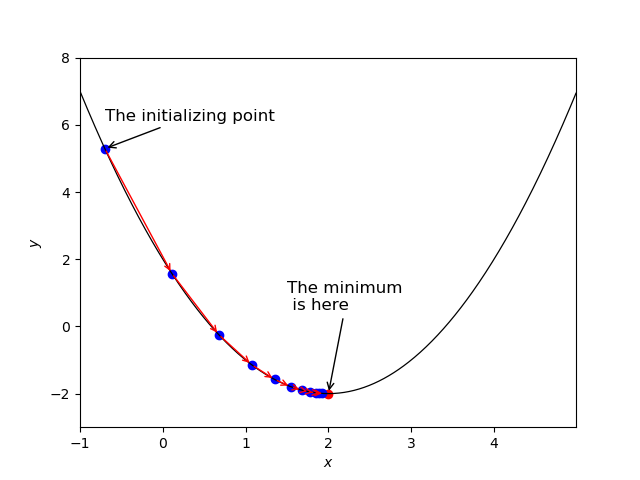
\includegraphics{fig1.png}
\caption{}
\end{figure}

    \begin{Verbatim}[commandchars=\\\{\}]
{\color{incolor}In [{\color{incolor}16}]:} \PY{o}{\PYZpc{}\PYZpc{}}\PY{k}{HTML}
         \PYZlt{}div align=\PYZdq{}middle\PYZdq{}\PYZgt{}
         \PYZlt{}video width=\PYZdq{}80\PYZpc{}\PYZdq{} controls\PYZgt{}
               \PYZlt{}source src=\PYZdq{}demo\PYZhy{}b.mp4\PYZdq{} type=\PYZdq{}video/mp4\PYZdq{}\PYZgt{}
         \PYZlt{}/video\PYZgt{}\PYZlt{}/div\PYZgt{}
\end{Verbatim}


    
    \begin{verbatim}
<IPython.core.display.HTML object>
    \end{verbatim}

    
    Reference:
https://gist.github.com/thanasi/ad31f798b747629e717bcebd2cad15cf

    \subsection{Exercise 1 (difficulty:
easy)}\label{exercise-1-difficulty-easy}

    given the function

\[
f(x)=3+x^3
\]

and its derivative

\[
\frac{df(x)}{dx} = 3x^2
\]

do the following

\begin{enumerate}
\def\labelenumi{\arabic{enumi}.}
\tightlist
\item
  Evaluate the derivative at the point 5, 6 and 10
\item
  Plot the derivative function and the function together and interpret
  the two functions.
\end{enumerate}

    \subsection{Exercise 2 (difficulty:
FUN)}\label{exercise-2-difficulty-fun}

    Ignoring the conditions in which this is true, for a function \(f(x)\)
in one dimensions that are continous and differentiable in a specific
rage one can find the location of the minimum or maximum solving the
equation

\[
\frac{df(x)}{dx} = 0
\]

Given the function

\[
f(x) = 3x+x^2+2
\]

find numerically the minimum or maximum (and identify which one is)
using the equation

\[
\frac{df(x)}{dx} = 3+2x = 0
\]

    \subsection{Exercise 3 (difficulty: hard) - Gradient
Descent}\label{exercise-3-difficulty-hard---gradient-descent}

    Consider again the function given in the previous exercise

\[
f(x) = 3x+x^2+2
\]

consider the following numerical series

\[
a_{n+1} = a_n - \gamma \frac{df(a_n)}{dx}
\]

Check numerically that, starting from a random value for \(a_0\), the
sequence \(a_n\) converges to the minimum you found in the previous
exercise. Check the method with several values of \(\gamma\). What do
you observe for big or small values? Can you compare the speed of
convergence?

Try with the following values

\[\gamma = 0.001, 0.1, 1.0, 3.0\]

What do you observe?

\textbf{HINT}:

\[
\frac{df(x)}{dx} = 3+2x
\]

If you want to read more on this method you can check here:
https://en.wikipedia.org/wiki/Gradient\_descent

    \subsubsection{Solution}\label{solution}

    \begin{Verbatim}[commandchars=\\\{\}]
{\color{incolor}In [{\color{incolor}197}]:} \PY{k}{def} \PY{n+nf}{gd}\PY{p}{(}\PY{n}{an}\PY{p}{,} \PY{n}{gamma}\PY{p}{)}\PY{p}{:}
              \PY{k}{return} \PY{n}{an}\PY{o}{\PYZhy{}}\PY{n}{gamma}\PY{o}{*}\PY{p}{(}\PY{l+m+mf}{3.0}\PY{o}{+}\PY{l+m+mf}{2.0}\PY{o}{*}\PY{n}{an}\PY{p}{)}
\end{Verbatim}


    \begin{Verbatim}[commandchars=\\\{\}]
{\color{incolor}In [{\color{incolor}209}]:} \PY{c+c1}{\PYZsh{} Starting point}
          \PY{n}{a0} \PY{o}{=} \PY{l+m+mi}{2}
          \PY{n}{gamma} \PY{o}{=} \PY{l+m+mf}{0.1}
          
          \PY{n}{a} \PY{o}{=} \PY{p}{[}\PY{n}{a0}\PY{p}{]}
          \PY{n}{n} \PY{o}{=} \PY{l+m+mi}{30} \PY{c+c1}{\PYZsh{} number of iteration}
          \PY{c+c1}{\PYZsh{} Loop}
          \PY{k}{for} \PY{n}{i} \PY{o+ow}{in} \PY{n+nb}{range} \PY{p}{(}\PY{l+m+mi}{1}\PY{p}{,}\PY{n}{n}\PY{p}{)}\PY{p}{:}
              \PY{n}{a}\PY{o}{.}\PY{n}{append}\PY{p}{(}\PY{n}{gd}\PY{p}{(}\PY{n}{a}\PY{p}{[}\PY{n}{i}\PY{o}{\PYZhy{}}\PY{l+m+mi}{1}\PY{p}{]}\PY{p}{,}\PY{n}{gamma}\PY{p}{)}\PY{p}{)}
              
          \PY{n+nb}{print}\PY{p}{(}\PY{l+s+s2}{\PYZdq{}}\PY{l+s+s2}{Expected values is}\PY{l+s+s2}{\PYZdq{}}\PY{p}{,} \PY{o}{\PYZhy{}}\PY{l+m+mf}{3.0}\PY{o}{/}\PY{l+m+mf}{2.0}\PY{p}{)}
          \PY{n+nb}{print}\PY{p}{(}\PY{l+s+s2}{\PYZdq{}}\PY{l+s+s2}{Algorithm estimation after}\PY{l+s+s2}{\PYZdq{}}\PY{p}{,}\PY{n}{n}\PY{p}{,}\PY{l+s+s2}{\PYZdq{}}\PY{l+s+s2}{iterations is}\PY{l+s+s2}{\PYZdq{}}\PY{p}{,} \PY{n}{a}\PY{p}{[}\PY{o}{\PYZhy{}}\PY{l+m+mi}{1}\PY{p}{]}\PY{p}{)}
\end{Verbatim}


    \begin{Verbatim}[commandchars=\\\{\}]
Expected values is -1.5
Algorithm estimation after 30 iterations is -1.4945840123281267

    \end{Verbatim}


    % Add a bibliography block to the postdoc
    
    
    
    \end{document}
